% Canonical paper: ICML 2026 Human-AI Co-Creativity workshop (non-archival).
% De-anonymized arXiv build. Reuses paper/sections/*.tex in the ICML
% two-column format. Build with .claude-tools/rebuild-latex.py.

\documentclass{article}

% Some PDF viewers (e.g. pdf.js) render default URW Times Type 1 fonts with
% broken kerning. cmap + T1 fontenc switch to encodings they handle correctly.
% Must come before microtype/icml2026.
\usepackage{cmap}
\usepackage[T1]{fontenc}

\usepackage{microtype}
\usepackage{graphicx}
\usepackage{subcaption}
\usepackage{booktabs}
\PassOptionsToPackage{hyphens}{url}  % allow URLs to break at hyphens/slashes (xurl unavailable in this TeX dist)
\usepackage{hyperref}

% Attempt to make hyperref and algorithmic work together better.
\newcommand{\theHalgorithm}{\arabic{algorithm}}

% Camera-ready: the workshop organizers' adapted style file. [accepted]
% de-anonymizes (shows the real author block) and prints the required
% first-page footnote "ICML'26 Workshop on Human-AI Co-Creativity, Seoul,
% South Korea." Do NOT override \ICML@appearing: the style file already
% carries the organizers' intended notice (workshop line + author copyright,
% correct for a non-archival workshop where authors retain copyright).
\usepackage[accepted]{icml2026_GenAICreativity}

\usepackage{amsmath}
\usepackage{amssymb}
\usepackage{amsthm}
\usepackage{enumitem}

\graphicspath{{../figures/}{../investigations/cross_mode_surprise_drop/figures/}}
\usepackage{pgfplots}
\usepgfplotslibrary{fillbetween}
\pgfplotsset{compat=1.18}
\usetikzlibrary{positioning, arrows.meta, fit, backgrounds, calc, shapes.geometric}

\newcommand{\E}{\mathbb{E}}
\newcommand{\KL}{D_{\mathrm{KL}}}
\newcommand{\pmi}{\mathrm{pmi}}
\newcommand{\TC}{\mathrm{TC}}

% Wrapper-aware switch for shared-section divergence (RW cross-ref noun;
% Figure 2 placement in §RLHF). Set to true in this workshop wrapper.
\newif\ifworkshop \workshoptrue

% Public project repository. Code and data live together — the dataset
% (Olmo generations + derived metrics) is under `results/rlhf_experiment/`.
\newcommand{\projectGithubUrl}{\url{https://github.com/AMindToThink/icl-diversity}}

% Script-generated inline scalars. Same source as original paper.
% Generated by scripts/build_paper_macros.py — DO NOT EDIT.
% Every inline numeric scalar referenced in the paper prose is defined here.
% Regenerate with: uv run python scripts/build_paper_macros.py
%
% Grouped by section for readability.

% --- Cross-mode pairwise (Sec 8.4) ---
\newcommand{\crossmodeAddOverpredMten}{622}
\newcommand{\crossmodeAddOverpredRatioMten}{10.6}
\newcommand{\crossmodeAinfFloor}{7.1}
\newcommand{\crossmodeAsymmetryMean}{5.6}
\newcommand{\crossmodeAsymmetryRatio}{3.0}
\newcommand{\crossmodeFracDropMone}{129.8}
\newcommand{\crossmodeFracOverpredMten}{2.2}
\newcommand{\crossmodeFracRatioMone}{1.0}
\newcommand{\crossmodeFracTotalDrop}{129}
\newcommand{\crossmodeGPTCrossDamageMten}{-3.4}
\newcommand{\crossmodeGPTDiagGainMten}{8.3}
\newcommand{\crossmodeGPTDiagMean}{83.0}
\newcommand{\crossmodeGPTDiagStd}{20.0}
\newcommand{\crossmodeGPTFirstStepDrop}{+4.9}
\newcommand{\crossmodeGPTNegColCount}{6}
\newcommand{\crossmodeGPTOffMean}{-3.7}
\newcommand{\crossmodeGPTOffPctPos}{30}
\newcommand{\crossmodeGPTOffStd}{2.9}
\newcommand{\crossmodeNumModes}{15}
\newcommand{\crossmodeNumOffPairs}{210}
\newcommand{\crossmodeObsDropMone}{127}
\newcommand{\crossmodeObsDropMten}{59}
\newcommand{\crossmodeObsDropMtenOneDec}{58.8}
\newcommand{\crossmodeQwenDiagMean}{60.5}
\newcommand{\crossmodeQwenDiagStd}{14.4}
\newcommand{\crossmodeQwenFirstStepDrop}{+7.8}
\newcommand{\crossmodeQwenNegColCount}{1}
\newcommand{\crossmodeQwenOffMean}{+1.9}
\newcommand{\crossmodeQwenOffPctPos}{64}
\newcommand{\crossmodeQwenOffStd}{2.5}
\newcommand{\crossmodeRDiag}{44.3}
\newcommand{\crossmodeROff}{1.4}

% --- Scaling / Llama (Sec 8.7) ---
\newcommand{\scalingFactorialProbPct}{4.2}
\newcommand{\scalingFracPosGPT}{30}
\newcommand{\scalingFracPosLlamaEightB}{44}
\newcommand{\scalingFracPosLlamaOneB}{25}
\newcommand{\scalingFracPosLlamaSeventyB}{63}
\newcommand{\scalingFracPosLlamaThreeB}{41}
\newcommand{\scalingFracPosQwen}{64}
\newcommand{\scalingNumLlamaModels}{4}
\newcommand{\scalingOffDiagGPT}{-3.7}
\newcommand{\scalingOffDiagLlamaEightB}{-1.2}
\newcommand{\scalingOffDiagLlamaOneB}{-4.9}
\newcommand{\scalingOffDiagLlamaSeventyB}{+2.1}
\newcommand{\scalingOffDiagLlamaThreeB}{-1.4}
\newcommand{\scalingOffDiagQwen}{+1.9}
\newcommand{\scalingRCRsqGPT}{0.08}
\newcommand{\scalingRCRsqLlamaEightB}{0.13}
\newcommand{\scalingRCRsqLlamaOneB}{0.44}
\newcommand{\scalingRCRsqLlamaSeventyB}{0.09}
\newcommand{\scalingRCRsqLlamaThreeB}{0.67}
\newcommand{\scalingRCRsqQwen}{0.34}
\newcommand{\scalingRCSlopeGPT}{0.35}
\newcommand{\scalingRCSlopeLlamaEightB}{0.41}
\newcommand{\scalingRCSlopeLlamaOneB}{1.01}
\newcommand{\scalingRCSlopeLlamaSeventyB}{0.37}
\newcommand{\scalingRCSlopeLlamaThreeB}{1.11}
\newcommand{\scalingRCSlopeQwen}{0.84}
\newcommand{\scalingSymRsqGPT}{0.14}
\newcommand{\scalingSymRsqLlamaEightB}{0.19}
\newcommand{\scalingSymRsqLlamaOneB}{0.33}
\newcommand{\scalingSymRsqLlamaSeventyB}{0.02}
\newcommand{\scalingSymRsqLlamaThreeB}{0.37}
\newcommand{\scalingSymRsqQwen}{0.24}
\newcommand{\scalingSymSlopeGPT}{0.33}
\newcommand{\scalingSymSlopeLlamaEightB}{0.59}
\newcommand{\scalingSymSlopeLlamaOneB}{0.65}
\newcommand{\scalingSymSlopeLlamaSeventyB}{0.16}
\newcommand{\scalingSymSlopeLlamaThreeB}{0.69}
\newcommand{\scalingSymSlopeQwen}{0.46}

% --- Qwen3 comparison (App E / Sec 8.7) ---
\newcommand{\qwenThreeBinaryMeanDeltaAUC}{-0.013}
\newcommand{\qwenThreeBinaryTies}{0}
\newcommand{\qwenThreeBinaryTotal}{12}
\newcommand{\qwenThreeBinaryWinsQwenThree}{1}
\newcommand{\qwenThreeBinaryWinsQwenTwoFive}{11}
\newcommand{\qwenThreeConTestPromptGenDeltaAUC}{+0.005}
\newcommand{\qwenThreeDecTestLosses}{0}
\newcommand{\qwenThreeDecTestMeanDeltaRho}{+0.021}
\newcommand{\qwenThreeDecTestTies}{1}
\newcommand{\qwenThreeDecTestTotal}{6}
\newcommand{\qwenThreeDecTestWins}{5}

% --- Tevet external validation (Sec 7.5) ---
\newcommand{\tevetAnVsCxAnOCAMaxPct}{17.4}
\newcommand{\tevetAnVsCxAnOCAMinPct}{3.6}
\newcommand{\tevetCVsCxAnOCAMaxPct}{33.2}
\newcommand{\tevetCVsCxAnOCAMinPct}{-1.4}
\newcommand{\tevetCoherenceBpbHigh}{2.20}
\newcommand{\tevetCoherenceBpbLow}{0.65}
\newcommand{\tevetCoherenceCHigh}{0.64}
\newcommand{\tevetCoherenceCLow}{0.22}
\newcommand{\tevetCoherenceMeanC}{0.42}
\newcommand{\tevetCoherenceRespCount}{48705}
\newcommand{\tevetCoherenceSetCount}{9741}
\newcommand{\tevetConTestPromptGenCxAnAUC}{0.837}
\newcommand{\tevetConTestSetCount}{670}
\newcommand{\tevetCxAnVsSentBertOCAMaxPct}{21.0}
\newcommand{\tevetCxAnVsSentBertOCAMinPct}{3.7}
\newcommand{\tevetDecTestAnPromptGenRho}{+0.932}
\newcommand{\tevetDecTestAnRespGenRho}{+0.924}
\newcommand{\tevetDecTestAnStoryGenRho}{+0.779}
\newcommand{\tevetDecTestDistinctNPromptGenRho}{+0.917}
\newcommand{\tevetDecTestSetCount}{2979}
\newcommand{\tevetLastUptickPct}{61}
\newcommand{\tevetMcDivNugPromptGenCxAnAUC}{0.867}
\newcommand{\tevetMcDivNugPromptGenDdiscAUC}{0.303}
\newcommand{\tevetMcDivNugSetCount}{3069}
\newcommand{\tevetMcDivPromptGenAUC}{0.921}
\newcommand{\tevetMcDivPromptGenCxAnOCA}{0.846}
\newcommand{\tevetMcDivPromptGenCxAnRho}{+0.729}
\newcommand{\tevetMcDivPromptGenDistinctNOCA}{0.746}
\newcommand{\tevetMcDivPromptGenDistinctNRho}{+0.476}
\newcommand{\tevetMcDivPromptGenSentBertOCA}{0.897}
\newcommand{\tevetMcDivPromptGenSentBertRho}{+0.796}
\newcommand{\tevetMcDivSetCount}{6002}

% --- Mode count (Sec 8.3) ---
\newcommand{\modeCountAnMone}{9.3}
\newcommand{\modeCountAnMten}{77.8}
\newcommand{\modeCountCxAnPearsonGPT}{0.98}
\newcommand{\modeCountCxAnPearsonQwen}{0.99}
\newcommand{\modeCountMMax}{10}
\newcommand{\modeCountNDraws}{1000}
\newcommand{\modeCountNResponses}{20}
\newcommand{\modeCountPoolSize}{50}

% --- Permutation sensitivity (Sec 8.6) ---
\newcommand{\permSensGPTMisranked}{2}
\newcommand{\permSensHighPerm}{100}
\newcommand{\permSensLowPerm}{3}
\newcommand{\permSensNumScenarios}{5}
\newcommand{\permSensQwenMisranked}{2}

% --- Scenario validation (Sec 3 Table 1 / App C.2) ---
\newcommand{\scenarioMixedGptDCan}{0.52}
\newcommand{\scenarioMixedQwenDCan}{0.41}
\newcommand{\scenarioMultiIncoherentGptDCan}{0.19}
\newcommand{\scenarioMultiIncoherentQwenDCan}{0.29}
\newcommand{\scenarioMultiModeGptDCan}{0.26}
\newcommand{\scenarioMultiModeQwenDCan}{0.19}
\newcommand{\scenarioOneModeGptDCan}{0.10}
\newcommand{\scenarioOneModeQwenDCan}{0.09}
\newcommand{\scenarioPureNoiseGptDCan}{0.04}
\newcommand{\scenarioPureNoiseQwenDCan}{0.05}

% --- Structural redundancy (draft sections/07_9_structural_redundancy.tex) ---
\newcommand{\framesQwenCosFramesOne}{0.32}
\newcommand{\framesQwenCosFramesTwenty}{0.21}
\newcommand{\framesQwenCosParaphrase}{0.81}
\newcommand{\framesQwenDropFramesOne}{0.546}
\newcommand{\framesQwenDropFramesOneSd}{0.088}
\newcommand{\framesQwenDropFramesTwenty}{0.739}
\newcommand{\framesQwenDropFramesTwentySd}{0.097}
\newcommand{\framesQwenDropParaphrase}{0.404}
\newcommand{\framesQwenDropParaphraseSd}{0.101}
\newcommand{\framesQwenNDraws}{20}
\newcommand{\framesQwenNResponses}{20}
\newcommand{\framesQwenNormDCanonical}{0.80}
\newcommand{\framesQwenNormDFramesOne}{0.49}
\newcommand{\framesQwenNormDistinctCanonical}{0.94}
\newcommand{\framesQwenNormDistinctFramesOne}{0.49}
\newcommand{\framesQwenNormSentBertCanonical}{0.97}
\newcommand{\framesQwenNormSentBertFramesOne}{0.82}
\newcommand{\framesQwenNumFrames}{20}
\newcommand{\framesQwenRhoD}{+0.601}
\newcommand{\framesQwenRhoDistinct}{+0.894}
\newcommand{\framesQwenRhoSentBert}{+0.787}
\newcommand{\posPatternAOneCanon}{2.192}
\newcommand{\posPatternAOneCanonSd}{0.240}
\newcommand{\posPatternAOneDiffP}{0.00069}
\newcommand{\posPatternAOneDiffSe}{0.068}
\newcommand{\posPatternAOneGapAbs}{0.252}
\newcommand{\posPatternAOneScram}{2.444}
\newcommand{\posPatternAOneScramSd}{0.184}
\newcommand{\posPatternAnCanon}{1.295}
\newcommand{\posPatternAnCanonSd}{0.187}
\newcommand{\posPatternAnDiff}{-0.174}
\newcommand{\posPatternAnDiffP}{0.0024}
\newcommand{\posPatternAnDiffSe}{0.053}
\newcommand{\posPatternAnGapAbs}{0.174}
\newcommand{\posPatternAnScram}{1.469}
\newcommand{\posPatternAnScramSd}{0.148}
\newcommand{\posPatternBytesCanon}{48.9}
\newcommand{\posPatternBytesScram}{49.2}
\newcommand{\posPatternCohCanon}{0.221}
\newcommand{\posPatternCohDiff}{+0.031}
\newcommand{\posPatternCohDiffPLtPow}{21}
\newcommand{\posPatternCohScram}{0.191}
\newcommand{\posPatternCosCanon}{0.221}
\newcommand{\posPatternCosDiffP}{0.11}
\newcommand{\posPatternCosScram}{0.227}
\newcommand{\posPatternCountNouns}{3}
\newcommand{\posPatternCountPreps}{2}
\newcommand{\posPatternCountVerbs}{1}
\newcommand{\posPatternDCanon}{0.286}
\newcommand{\posPatternDDiffP}{0.59}
\newcommand{\posPatternDScram}{0.280}
\newcommand{\posPatternDistinctCanon}{0.938}
\newcommand{\posPatternDistinctDiff}{-0.0061}
\newcommand{\posPatternDistinctDiffPLtPow}{4}
\newcommand{\posPatternDistinctLowerDiff}{-0.0002}
\newcommand{\posPatternDistinctLowerP}{0.88}
\newcommand{\posPatternDistinctScram}{0.945}
\newcommand{\posPatternDropCanon}{0.597}
\newcommand{\posPatternDropCanonSd}{0.104}
\newcommand{\posPatternDropDiffP}{0.81}
\newcommand{\posPatternDropScram}{0.604}
\newcommand{\posPatternDropScramSd}{0.073}
\newcommand{\posPatternLearnedPctCanon}{40}
\newcommand{\posPatternLearnedPctScram}{40}
\newcommand{\posPatternNDraws}{20}
\newcommand{\posPatternNResponses}{40}
\newcommand{\posPatternNumNouns}{197}
\newcommand{\posPatternNumOrders}{60}
\newcommand{\posPatternNumPreps}{35}
\newcommand{\posPatternNumVerbs}{106}
\newcommand{\posPatternOrderBits}{5.91}
\newcommand{\posPatternOrderBitsPerByte}{0.12}
\newcommand{\posPatternSlotsTotal}{6}


\icmltitlerunning{\textquotedblleft I've Seen How This Goes\textquotedblright: Characterizing Diversity via Progressive Conditional Surprise}

\begin{document}

\twocolumn[
\icmltitle{\textquotedblleft I've Seen How This Goes\textquotedblright: Characterizing the Diversity of LLM Generations and Human Writing via Progressive Conditional Surprise}

\icmlsetsymbol{equal}{*}

\begin{icmlauthorlist}
\icmlauthor{Matthew Khoriaty}{era}
\icmlauthor{David Williams-King}{era}
\icmlauthor{Shi Feng}{gwu}
\end{icmlauthorlist}

\icmlaffiliation{era}{ERA Fellowship}
\icmlaffiliation{gwu}{George Washington University}

\icmlcorrespondingauthor{Matthew Khoriaty}{matthewkhoriaty@gmail.com}

\icmlkeywords{diversity, language models, mode collapse, in-context learning, evaluation, creativity}

\vskip 0.3in
]

\printAffiliationsAndNotice{}

\begin{abstract}
Measuring the diversity of creative outputs is central to evaluating post-training mode collapse, comparing decoding strategies, and quantifying creative behavior in both AI and human writing.
Existing diversity metrics rely on embedding distances or $n$-gram statistics, both of which conflate genuine content diversity with lexical or representational artefacts.
We propose $D_{Ca_n} = C \times a_n$: a per-byte score read off the per-token log-probabilities of a base model $\theta$ in a \emph{single forward pass} per permutation, with no embedding model, no reference corpus, and no human labels.
The same pipeline scores AI samples and human-written response sets, with diversity treated as a property of (responses, prompt, scoring model) rather than how the responses were produced.
On Tevet and Berant's human-grounded McDiv benchmark, $D_{Ca_n}$ reaches ROC AUC \tevetMcDivPromptGenAUC{} on McDiv prompt\_gen, at the level of the strongest embedding baseline.
On the OLMo-2-7B post-training pipeline, $D_{Ca_n}$ drops monotonically across the base $\to$ SFT $\to$ DPO $\to$ RLVR stages, detecting the diversity loss that creative-writing applications care about.

\end{abstract}

% --- Main body (target 4-8 pages; trimmed via Phase 3 workshop variants) ---
% Phase 3 will swap each shared-section \input{} below for a *_workshop.tex
% variant per the plan in paper/human-ai-creativity-workshop.md.

\section{Motivation}\label{sec:motivation}

The possibility for diverse outputs is necessary, but not sufficient, for creativity.
Machine learning researchers that study creativity
%Creativity researchers
routinely need to compare the diversity of outputs across generation processes: post-training stages of the same base model (mode collapse), decoding strategies (what does temperature trade off against?), prompting interventions (which prompts have a wide response distribution?), and human-AI hybrid pipelines (would AI use cause human-AI writing to be less creative?).
Existing diversity metrics rely on embedding distances \citep{du2019boosting} or surface-level $n$-gram statistics, both of which lack a human-like ability to recognize arbitrary patterns when those patterns differ from their training data or surface similarities, respectively (\ifworkshop Section\else Appendix\fi~\ref{sec:related}).
A complementary line of work applies information theory directly: Maximum Mutual Information decoding \citep{li2016diversity} and Adversarial Information Maximization \citep{zhang2018aim} optimise pairwise mutual information between input and response, but as a training or decoding objective rather than an evaluation-time diagnostic.
We propose a new approach to measuring diversity using in-context learning, of which the ``Decan'' metric $D_{Ca_n} = C \times a_n$ is the working instance we evaluate: it scores AI samples and human-written response sets through the same pipeline of per-byte log-probabilities of a base model $\theta$, in a \emph{single forward pass} over the concatenated responses (Figure~\ref{fig:pipeline}).
There is no embedding model, no reference corpus, no human labels, no auxiliary classifier.
The approach uses only the per-token probabilities $\theta$ already produces.

The intuition is that if responses from a policy $\pi$ are diverse, seeing one should not help $\theta$ predict the next; if they are repetitive or constrained to a few modes, conditioning on earlier responses should sharply reduce $\theta$'s surprise at later ones.
We exploit the in-context learning capability described by \citet{brown2020language}, applied here as a measurement lens rather than as a few-shot-prompting setup.
The progressive conditional surprise curve $a_k$ (the per-byte cross-entropy of the $k$-th response given the previous $k{-}1$) captures this signal directly, and its last point is $a_n$ (Section~\ref{sec:progressive-conditioning}).
A separate coherence term $C = 1/\mathrm{PPL}_\theta(\pi, p)$, the reciprocal of the geometric-mean per-byte perplexity that $\theta$ assigns to each response individually, prevents pure noise from registering as ``diverse'' (Section~\ref{sec:coherence}).
The product $D_{Ca_n} = C \times a_n$ is the working scalar we adopt; it is plausibility-weighted residual diversity in bits per byte.
We validate it against Tevet and Berant's human-grounded diversity benchmark (Section~\ref{sec:tevet}) and on the OLMo-2-7B post-training pipeline (Section~\ref{sec:rlhf-experiment}), and release a working open-source implementation alongside.\footnote{Code and data: \projectGithubUrl}
The metric measures diversity as $\theta$ perceives it: outputs differing only in ways $\theta$ cannot distinguish in context appear less diverse.
This relativity gives the metric the potential to tighten as base models improve (see Appendix~\ref{app:qwen3-comparison} for a preliminary scaling experiment).

\begin{figure*}[tbp]
\centering
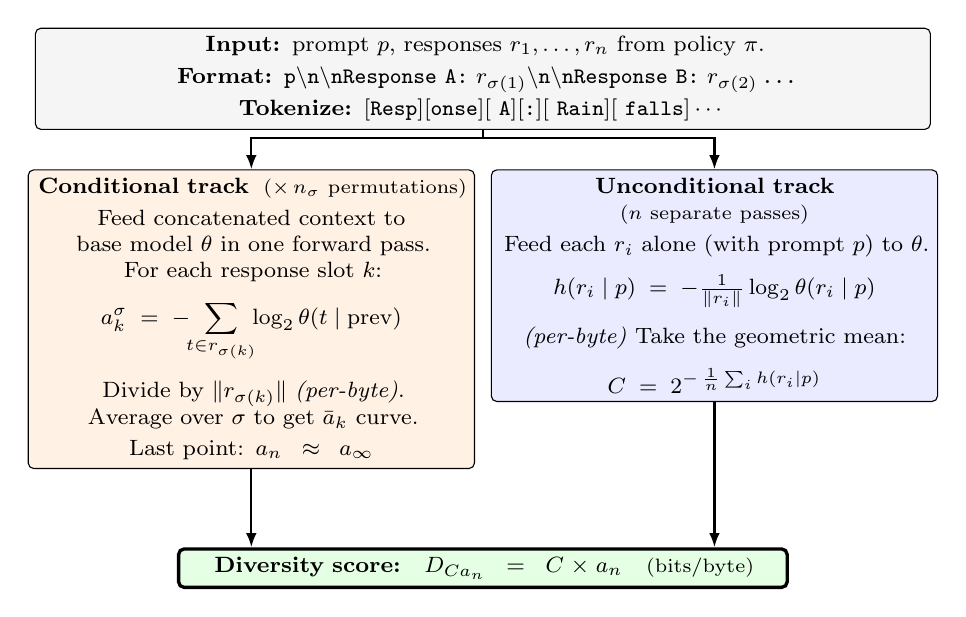
\begin{tikzpicture}[
    font=\footnotesize,
    box/.style={draw, rounded corners=2pt, align=center, inner sep=3pt},
    stage/.style={box, fill=gray!8},
    cond/.style={box, fill=orange!10},
    uncond/.style={box, fill=blue!8},
    final/.style={box, fill=green!10, very thick},
    arrow/.style={-{Latex[length=1.8mm]}, thick},
    node distance=2mm and 4mm,
]

% --- INPUT + FORMAT (combined, top) ---
\node[stage, text width=0.92\textwidth] (input) {
    \textbf{Input:} prompt $p$, responses $r_1,\ldots,r_n$ from policy $\pi$.\\[2pt]
    \textbf{Format:} \texttt{p\textbackslash n\textbackslash nResponse A: $r_{\sigma(1)}$\textbackslash n\textbackslash nResponse B: $r_{\sigma(2)}$\,\ldots}\\[2pt]
    \textbf{Tokenize:} $[\texttt{Resp}][\texttt{onse}][\texttt{ A}][\texttt{:}][\texttt{ Rain}][\texttt{ falls}]\cdots$
};

% --- CONDITIONAL TRACK (LEFT) ---
\node[cond, below left=5mm and 1mm of input.south, text width=0.45\textwidth, anchor=north east] (cond) {
    \textbf{Conditional track} \;{\scriptsize ($\times\,n_\sigma$ permutations)}\\[2pt]
    Feed concatenated context to base model $\theta$ in one forward pass.\\
    For each response slot $k$:
    \[ a_k^\sigma \;=\; -\!\!\sum_{t \in r_{\sigma(k)}}\!\!\log_2 \theta(t \mid \mathrm{prev}) \]
    Divide by $\|r_{\sigma(k)}\|$ \emph{(per-byte)}.\\
    Average over $\sigma$ to get $\bar{a}_k$ curve.\\[2pt]
    Last point: $a_n \approx a_\infty$
};

% --- UNCONDITIONAL TRACK (RIGHT) ---
\node[uncond, below right=5mm and 1mm of input.south, text width=0.45\textwidth, anchor=north west] (unc) {
    \textbf{Unconditional track} \;{\scriptsize ($n$ separate passes)}\\[2pt]
    Feed each $r_i$ alone (with prompt $p$) to $\theta$.
    \[ h(r_i\mid p) \;=\; -\tfrac{1}{\|r_i\|}\log_2 \theta(r_i \mid p) \]
    \emph{(per-byte)} Take the geometric mean:
    \[ C \;=\; 2^{-\,\frac{1}{n}\sum_i h(r_i\mid p)} \]
};

% Arrows from input down to each track
\draw[arrow] (input.south) -- ++(0,-1mm) -| (cond.north);
\draw[arrow] (input.south) -- ++(0,-1mm) -| (unc.north);

% --- FINAL FORMULA ---
\node[final, below=4mm of input, text width=0.62\textwidth, yshift=-49mm] (out) {
    \textbf{Diversity score:}\quad $D_{Ca_n} \;=\; C \times a_n$\quad{\scriptsize(bits/byte)}
};

% Arrows from each track straight down into the final box
\draw[arrow] (cond.south) -- (cond.south |- out.north);
\draw[arrow] (unc.south)  -- (unc.south |- out.north);

\end{tikzpicture}
\caption{The diversity-metric pipeline.
Given prompt $p$ and $n$ responses from policy $\pi$, we format them with response labels (``Response A:'', ``Response B:'', \ldots) and tokenize.
The \textcolor{orange!70!black}{\textbf{conditional track}} (left) feeds the concatenated context to the base model $\theta$ in a single forward pass per permutation $\sigma$, extracts per-response total surprise, divides by each response's UTF-8 byte count, and averages over permutations to get $\bar a_k$.
Its last point is $a_n$.
The \textcolor{blue!70!black}{\textbf{unconditional track}} (right) scores each $r_i$ independently against the prompt alone, again per-byte; the geometric mean of these surprises defines coherence $C = 1/\mathrm{PPL}_\theta(\pi, p)$, the reciprocal of the geometric-mean per-byte perplexity.
The product $D_{Ca_n} = C \times a_n$ measures plausibility-weighted residual diversity (bits/byte).
Formal definitions: Sections~\ref{sec:setup-notation}, \ref{sec:progressive-conditioning}, \ref{sec:coherence}, \ref{sec:scalar}.}
\label{fig:pipeline}
\end{figure*}


\section{Setup and Notation}\label{sec:setup-notation}

We use the following notation:
\begin{itemize}[nosep]
    \item $p$ be a prompt,
    \item $\pi$ be the policy under evaluation,
    \item $r_1, r_2, \ldots, r_n \sim \pi(\cdot \mid p)$ be $n$ i.i.d.\ responses sampled from $\pi$,
    \item $\theta$ be a trusted base model from which we can obtain per-token log-probabilities,
    \item $|r|_{\mathrm{tok}}$ denote the number of tokens in response $r$,
    \item $\|r\|$ denote the number of bytes in the UTF-8 encoding of response $r$.
\end{itemize}

We define the \textbf{cross-entropy} (total surprise) of a response $r$ under $\theta$:
\begin{equation}\label{eq:total-xent}
    -\log_2 \theta(r \mid p) = \sum_{t=1}^{|r|_{\mathrm{tok}}} -\log_2 \theta(r^t \mid r^{<t}, p)
\end{equation}
where $r^t$ is the $t$-th token and $r^{<t}$ the preceding tokens.
Units: bits.\footnote{Throughout, ``bits'' refers to self-information in $\log_2$ units, identical to the ``shannon'' (Sh) of IEC 80000-13.
We use ``bits'' to match standard usage in the information-theory literature.} This is the total surprise of the response under $\theta$, a function of the string and of $\theta$'s distribution but not of $\theta$'s tokenizer (since the chain rule yields the same total regardless of how the sequence is factored).

Similarly, the \textbf{conditional cross-entropy} given previous responses $r_{<k} = (r_1, \ldots, r_{k-1})$ is $-\log_2 \theta(r_k \mid r_{<k}, p)$ (bits).

For the coherence term and diversity scores (Sections~\ref{sec:coherence} and \ref{sec:scalar}), we also use the \textbf{per-byte cross-entropy rate}:
\begin{equation}\label{eq:pertok}
    h_\theta(r \mid p) = \frac{-\log_2 \theta(r \mid p)}{\|r\|}
\end{equation}
Units: bits/byte.
We adopt this per-byte rate because it works better than total bits in our experiments; we have not investigated why.
Normalising by byte count rather than token count keeps the rate independent of $\theta$'s tokenizer when comparing base models with different vocabularies.

In practice, computing $\theta(r_k \mid r_{<k}, p)$ requires feeding $\theta$ a formatted context containing the prompt and all previous responses (see Section~\ref{sec:practical}).


\section{Method}\label{sec:method}

This section defines the three quantities the workshop variant uses: the progressive conditional surprise curve $a_k$, the coherence term $C$, and the scalar score $D_{Ca_n} = C \times a_n$.
The full information-theoretic motivation, the alternative excess-entropy summary $E$, the coherence-heterogeneity diagnostic $\sigma_\ell$, and the cross-mode learning analysis appear in Appendices~\ref{app:k0-derivation}--\ref{app:qwen3-comparison}.

\subsection{Progressive Conditional Surprise}\label{sec:progressive-conditioning}

Given prompt $p$ and $n$ responses $r_1, \ldots, r_n$ from policy $\pi$, define
\begin{equation}\label{eq:ak}
    a_k = -\log_2 \theta(r_k \mid r_{<k}, p) \quad \text{for } k = 1, \ldots, n,
\end{equation}
the total surprise of the $k$-th response under base model $\theta$ given the previous $k{-}1$ responses.
The sequence $(a_1, \ldots, a_n)$ is the \textbf{progressive conditional surprise curve}.
We normalize each $a_k$ by the byte count $\|r_k\|$ to get a per-byte (bits/byte) curve that is independent of $\theta$'s tokenizer.
All quantities below are per-byte unless otherwise stated.

The intuition is that as $\theta$ sees more responses from $\pi$, the conditional surprise drops if the responses share patterns ($\theta$'s in-context learning picks up on modes, stylistic regularities, topic patterns) and stays flat if they do not.
For a policy with rich coherent diversity the curve declines and levels off at a positive floor; for a policy producing one repeated mode the curve drops sharply to near zero; for pure noise the curve stays roughly constant at a high value.

In practice we average $a_k$ over uniformly random permutations of the response ordering (so each position averages over all responses and the curve reflects only how $\theta$'s predictions improve with more context, not which response happened to land in slot $k$).
The asymptotic floor is taken to be the last observed point: $a_\infty \approx a_n$.
No fitting or extrapolation step is involved.

\subsection{The Coherence Term}\label{sec:coherence}

The curve alone cannot distinguish a policy producing rich coherent diversity from one producing several individually incoherent modes.
For both, $\theta$ may learn the mode structure from context (so $a_k$ drops meaningfully) and end up at a similar floor.
The distinguishing signal lies in how plausible $\theta$ finds each individual response, independent of the others.

Let $h_\theta(r \mid p) = -\frac{1}{\|r\|}\log_2 \theta(r \mid p)$ be the per-byte cross-entropy of response $r$ under $\theta$ conditioned on the prompt alone.
Define \textbf{coherence} as the geometric mean of the per-byte probabilities:
\begin{equation}\label{eq:coherence}
    C = 2^{-\frac{1}{n}\sum_{i=1}^{n} h_\theta(r_i \mid p)} = \frac{1}{\mathrm{PPL}_\theta(\pi, p)},
\end{equation}
the reciprocal of the geometric-mean per-byte perplexity that $\theta$ assigns to the responses individually.\footnote{For scale, GPT-3 davinci on The Pile \citep{gao2020pile} scored $\sim$0.72 bits/byte and GPT-2 XL $\sim$1.05 bits/byte, giving $C \approx 0.61$ and $C \approx 0.49$ respectively; stronger base models reach lower bits/byte and correspondingly higher $C$.}
Geometric averaging (rather than arithmetic) is what gives $C$ the desired suppression: a single fluent response cannot rescue a set in which the rest are incoherent, because $C$ is driven toward zero by any sample with high per-byte cross-entropy.

\subsection{The Diversity Score}\label{sec:scalar}

The scalar score is the product:
\begin{equation}\label{eq:D-Can}
    D_{Ca_n} = C \times a_n \quad \text{(bits/byte).}
\end{equation}
It can be read as ``how many bits of surprise per byte remain after $\theta$ has learned everything it can from the other responses, weighted by output plausibility.''
The intended edge-case behaviors are summarized in Table~\ref{tab:edge-cases}; empirical metric values on synthetic instances of each scenario appear in Appendix~\ref{sec:scenario-validation} (Table~\ref{tab:scenarios}).

\begin{table}[t]
\centering
\small
\caption{Intended edge-case behavior of $D_{Ca_n} = C \times a_n$ on the five appendix scenarios (Appendix~\ref{sec:scenario-validation}).
The product correctly suppresses pure noise and incoherent multi-mode (via $C$) and correctly suppresses one-mode sets (via $a_n$); multi-mode coherent is the intended winner.
Empirical numbers under GPT-2 and Qwen2.5-3B appear in Table~\ref{tab:scenarios}.}
\label{tab:edge-cases}
\begin{tabular}{@{}lccc@{}}
\toprule
Scenario              & $C$  & $a_n$ & $D_{Ca_n}$       \\
\midrule
Pure noise            & low  & high  & low (via $C$)    \\
Multi-mode incoherent & low  & high  & low (via $C$)    \\
Multi-mode coherent   & high & high  & \textbf{high}    \\
One-mode              & high & low   & low (via $a_n$)  \\
Mixed                 & mid  & high  & mid              \\
\bottomrule
\end{tabular}
\end{table}

The score depends on $p$, $\pi$'s responses, and $\theta$.
Diversity is therefore a property of (responses, prompt, scoring model), not of the policy in isolation: the same response set can score differently under a stronger or weaker $\theta$.
This is by design: $\theta$'s in-context learning capability is the lens through which diversity is measured, and the score sharpens automatically as base models improve.
When comparing policies across a prompt suite, $D_{Ca_n}$ can be averaged over prompts or differenced; see Appendix~\ref{app:aggregation}.


\section{Related Work}\label{sec:related}

\paragraph{Sampling diversity metrics.} Work on decoding-time diversity typically operates at the surface level: $n$-gram overlap \citep{li2016diversity} and self-BLEU \citep{zhu2018texygen}.
Our approach operates at the distributional level and can distinguish policies that produce lexically varied but semantically redundant outputs.

\paragraph{Diversity evaluation benchmarks.}
\citet{tevet2020evaluating} introduced a systematic framework for evaluating diversity metrics, with their McDiv benchmark providing human-labeled response sets at two diversity levels.
We use McDiv for validation (Section~\ref{sec:tevet}), though we identify a construction confound in how its low-diversity sets are produced (Appendix~\ref{app:confound}).
More recent work has revisited the meta-evaluation problem.
NoveltyBench \citep{zhang2025noveltybench} defines diversity through pairwise functional equivalence rather than binary labels, training a DeBERTa classifier to group generations into equivalence classes and computing a \emph{Distinct}$_k$ score (the number of meaningfully different outputs in $k$ samples), conceptually close to our mode count.
However, their ground truth is itself a trained classifier (79\% accuracy), making it unclear whether correlation with their labels validates a metric or merely measures agreement between two model-based scores.
\citet{zhang2025commonsense} conduct a meta-evaluation of diversity metrics for constrained commonsense generation, using GPT-4o as an annotator in place of crowd workers.
\citet{guo2024linguistic} benchmark linguistic diversity of LLMs, building on Tevet and Berant's framework with a broader set of generation tasks.

\paragraph{Perplexity.} The coherence term $C = 1/\mathrm{PPL}$ (Section~\ref{sec:coherence}) connects our framework to the standard language modeling evaluation metric.
The primary diversity score $D_{Ca_n} = C \times a_n$ operates in bits/byte, weighting the residual surprise floor by output plausibility.

\paragraph{Coherence as a signal.} Our coherence term $C$ uses the base model's predictive distribution as an unsupervised quality signal.
This connects to a broader line of work using model-internal coherence without external supervision: \citet{qiu2026selfimprovement} show theoretically that feedback-free self-improvement methods work by optimizing coherence (compressibility of context-to-behavior mappings), and \citet{wen2025unsupervised} use internal coherence maximization to elicit capabilities from language models.
Our framework leverages a related insight: the base model's ability to compress responses in context provides a meaningful signal about their diversity structure.

\paragraph{Embedding-based diversity.} \citet{du2019boosting} introduced the embedding-based approach, clustering sentence embeddings of generated responses with $k$-means and reporting cluster inertia as the diversity score; subsequent work has explored alternative geometric statistics over embedded responses.
These approaches are complementary to ours: they capture semantic distance in a learned representation space, while our metric captures statistical independence under a generative model.
The approaches may disagree when $\theta$'s in-context learning captures structure invisible to the embedding model, or vice versa.

\paragraph{Output collapse in RL training.} \citet{wang2025ragen} document an ``Echo Trap'' pattern during multi-turn agent RL: early-stage agents produce varied symbolic reasoning, then collapse to deterministic templates as training proceeds.
They detect this collapse using within-prompt reward standard deviation as an early-warning signal, a proxy that relies on the reward distinguishing degenerate outputs from diverse ones.
The $a_k$ framework provides a text-level alternative: collapse should appear as a drop in $a_n$ on the agent's own outputs, independent of reward structure. A downside of using the $a_k$ framework is that it is unconnected from a downstream task. Responses can both be "diverse" as measured by $a_k$-based metrics and fail uniformly.

\paragraph{Excess entropy.} The $a_k$ curve also admits an excess-entropy summary related to the computational mechanics literature \citep{crutchfield2003regularities}; see Appendix~\ref{app:excess-entropy}.
We found it empirically inferior to $D_{Ca_n}$ on Tevet and Berant's diversity-eval benchmark \citep{tevet2020evaluating}.
\section{Tevet--Berant Diversity-Eval: Human-Grounded Validation}\label{sec:tevet}

A diversity metric should be tested against human judgements on a standardized eval; \citet{tevet2020evaluating} provide both.
Their McDiv and ConTest datasets pair human-grounded diversity labels with a fixed comparison protocol (Spearman $\rho$ and OCA: \emph{optimal classification accuracy}, the best accuracy achievable by a one-dimensional threshold separating low- and high-diversity sets), the standard methodology for ranking diversity metrics against human judgements.
The response sets are written by Mechanical Turk workers, and for the McDiv\_nuggets subset the high/low label is fixed by the construction protocol itself: a worker writes five different continuations (the high-diversity set), then self-selects one of those continuations and paraphrases it five times (the low-diversity set; see Appendix~\ref{app:confound} for the full protocol and a construction-confound caveat).
We run $D_{Ca_n}$ through this evaluation pipeline.

\paragraph{Setup.} We use Qwen2.5-3B (base) with 50 permutations in completion format on the released no\_hds splits: \tevetMcDivSetCount{} McDiv sets, \tevetMcDivNugSetCount{} McDiv\_nuggets sets, and \tevetConTestSetCount{} ConTest sets, each with 5 worker-written responses per set and a binary high/low diversity label.
We follow Tevet and Berant in reporting Spearman $\rho$ and OCA, and additionally report ROC AUC (the natural metric for binary classification).

\begin{table*}[t]
\centering
\caption{ConTest results: Spearman $\rho$ and OCA between a set's diversity class and each metric score.
Baselines from Tevet's pre-computed metrics; $C \!\times\! a_n$ and $a_n$ are ours (Qwen2.5-3B, 50 permutations, per-byte).
Best result per task in bold.}
\label{tab:contest}
\small
% Generated by: scripts/analyze_c_ainf.py --run-tag qwen25_completion_v3
% Baseline source: diversity-eval/data/with_metrics/
\begin{tabular}{@{}l rr rr rr@{}}
\toprule
& \multicolumn{2}{c}{prompt\_gen} & \multicolumn{2}{c}{resp\_gen} & \multicolumn{2}{c}{story\_gen} \\
\cmidrule(lr){2-3} \cmidrule(lr){4-5} \cmidrule(lr){6-7}
Metric & $\rho$ & OCA & $\rho$ & OCA & $\rho$ & OCA \\
\midrule
\multicolumn{7}{@{}l}{\textit{ConTest (200, with\_hds)}} \\[2pt]
$C \!\times\! a_n$ (ours) & +0.584 & 0.785 & +0.391 & 0.668 & +0.686 & 0.828 \\
$a_n$ (ours) & +0.444 & 0.715 & +0.274 & 0.641 & +0.387 & 0.684 \\
SentBERT & \textbf{+0.682} & 0.815 & \textbf{+0.591} & \textbf{0.791} & \textbf{+0.770} & \textbf{0.896} \\
BERTsts & +0.646 & \textbf{0.820} & +0.463 & 0.714 & +0.601 & 0.780 \\
distinct-$n$ & +0.333 & 0.675 & +0.346 & 0.677 & +0.573 & 0.772 \\
\midrule
\multicolumn{7}{@{}l}{\textit{McDiv\_nuggets ($\sim$1K, no\_hds)}} \\[2pt]
$C \!\times\! a_n$ (ours) & +0.636 & 0.785 & +0.345 & 0.649 & +0.317 & 0.634 \\
$a_n$ (ours) & +0.487 & 0.705 & +0.225 & 0.619 & +0.124 & 0.557 \\
SentBERT & \textbf{+0.728} & \textbf{0.850} & \textbf{+0.532} & \textbf{0.758} & \textbf{+0.633} & \textbf{0.803} \\
BERTsts & +0.683 & 0.830 & +0.393 & 0.676 & +0.344 & 0.638 \\
distinct-$n$ & $-0.003$ & 0.514 & $-0.002$ & 0.507 & $-0.002$ & 0.510 \\
\midrule
\multicolumn{7}{@{}l}{\textit{McDiv (full, no\_hds, $\sim$2K)}} \\[2pt]
$C \!\times\! a_n$ (ours) & +0.729 & 0.846 & +0.500 & 0.724 & +0.523 & 0.717 \\
$a_n$ (ours) & +0.617 & 0.781 & +0.432 & 0.698 & +0.402 & 0.668 \\
SentBERT & \textbf{+0.796} & \textbf{0.897} & \textbf{+0.678} & \textbf{0.830} & \textbf{+0.753} & \textbf{0.867} \\
BERTsts & +0.780 & 0.893 & +0.614 & 0.781 & +0.571 & 0.740 \\
distinct-$n$ & +0.476 & 0.746 & +0.517 & 0.738 & +0.535 & 0.744 \\
\bottomrule
\end{tabular}

\end{table*}

\paragraph{Headline result.} On the binary tasks $D_{Ca_n}$ matches the strongest embedding baseline (Table~\ref{tab:contest}).
On McDiv prompt\_gen, $D_{Ca_n}$ reaches $\rho = \tevetMcDivPromptGenCxAnRho{}$ and OCA = \tevetMcDivPromptGenCxAnOCA{}, against SentBERT's $\rho = \tevetMcDivPromptGenSentBertRho{}$ and OCA = \tevetMcDivPromptGenSentBertOCA{}; the corresponding ROC AUC is \tevetMcDivPromptGenAUC{}.
Across the nine binary tasks, $D_{Ca_n}$'s OCA lags SentBERT by \tevetCxAnVsSentBertOCAMinPct\%--\tevetCxAnVsSentBertOCAMaxPct\%; it beats distinct-$n$ decisively on all three McDiv\_nuggets tasks (where distinct-$n$ is near chance) and trails it by 1--3 OCA points on three of the nine tasks where the labels are nearly shuffle-invariant.
The headline takeaway for this audience is that an information-theoretic, embedding-free metric reaches the same operating point as a sentence-embedding baseline on a human-grounded eval, with no embedding model, no reference corpus, and no human labels in the metric itself.

\paragraph{DecTest, included for completeness.} Tevet and Berant also release DecTest (Table~\ref{tab:dectest}), a diagnostic where the ``label'' is the sampling temperature used to generate each response set rather than a human judgement.
We include it for parity with the released benchmark only: temperature labels do not map onto creative-output diversity in any way that reflects the use cases in Section~\ref{sec:motivation}.
The raw $a_n$ achieves $\rho = \tevetDecTestAnPromptGenRho{}$ on prompt\_gen and $\rho = \tevetDecTestAnRespGenRho{}$ on resp\_gen, matching or exceeding all baselines.

\begin{table}[t]
\centering
\caption{DecTest results: Spearman $\rho$ between sampling temperature and each metric score (1000 samples, no\_hds).
Reported for parity with Tevet and Berant; the labels here are sampling temperatures rather than human judgements, so DecTest is not part of the framing for $D_{Ca_n}$.}
\label{tab:dectest}
\small
% Generated by: scripts/analyze_c_ainf.py --run-tag qwen25_completion_v3
% Baseline source: diversity-eval/data/with_metrics/
\begin{tabular}{@{}l rrr@{}}
\toprule
Metric & prompt\_gen & resp\_gen & story\_gen \\
\midrule
$C \!\times\! a_n$ (ours) & +0.847 & +0.771 & +0.763 \\
$a_n$ (ours) & \textbf{+0.932} & \textbf{+0.924} & \textbf{+0.779} \\
$C$ (ours) & $-0.727$ & $-0.813$ & $-0.547$ \\
distinct-$n$ & +0.917 & +0.894 & +0.758 \\
BERTScore & +0.878 & +0.874 & +0.694 \\
SentBERT & +0.747 & +0.801 & +0.645 \\
cos-sim & +0.873 & +0.895 & +0.712 \\
\bottomrule
\end{tabular}

\end{table}

\paragraph{Caveats.} The McDiv\_nuggets construction protocol introduces a confound: low-diversity sets are paraphrases of specific, dramatic endings that are intrinsically more surprising to the base model than typical high-diversity continuations.
Appendix~\ref{app:confound} documents the mechanism, the per-byte $a_1$ gap, and an evidence-by-length-bin breakdown showing the effect is content-driven not length-driven.
The $C$ weighting in $D_{Ca_n}$ helps on this benchmark partly for that confound-related reason; on settings without such a confound we expect $a_n$ to carry most of the signal.


% ============================================================================
% Workshop variant of the OLMo-2-7B RLHF case study.
% Differences from sections/07_6_rlhf.tex:
%   - Promoted from \subsection to \section (no §7 Experiments parent in
%     the workshop wrapper).
%   - One-paragraph framing intro added so this section is read as the
%     AI-side anchor (parallel to Tevet as the Human-side anchor).
%   - Cross-model comparison trimmed to a one-sentence pointer to the
%     appendix; full table and discussion live in sections/07_6_rlhf.tex
%     which is appendix-only in the workshop wrapper.
%   - Released-artifacts URL replaced with anonymous-mirror placeholder
%     for double-blind review (Phase 4 finalizes the workaround).
% ============================================================================

% Load generated macros BEFORE the section body so prose references resolve.
\IfFileExists{../results/rlhf_experiment/paper_macros_rlhf.tex}{%
  % Auto-generated by scripts/rlhf_experiment/5_analyze_and_figures.py

\newcommand{\olmoAlpacaBaseDMean}{0.488}
\newcommand{\olmoAlpacaSftDMean}{0.330}
\newcommand{\olmoAlpacaDpoDMean}{0.290}
\newcommand{\olmoAlpacaInstructDMean}{0.285}
\newcommand{\olmoAlpacaHoneAPbonf}{0.000}
\newcommand{\olmoAlpacaHoneADz}{1.614}
\newcommand{\olmoAlpacaHoneADiff}{0.158}
\newcommand{\olmoAlpacaHoneBPbonf}{0.000}
\newcommand{\olmoAlpacaHoneBDz}{0.577}
\newcommand{\olmoAlpacaHoneBDiff}{0.040}
\newcommand{\olmoAlpacaHoneCPbonf}{0.000}
\newcommand{\olmoAlpacaHoneCDz}{2.526}
\newcommand{\olmoAlpacaHoneCDiff}{0.202}
\newcommand{\olmoAlpacaHpaP}{0.000}
\newcommand{\olmoAlpacaHpaDz}{0.222}
\newcommand{\olmoAlpacaHpaDiff}{0.005}
\newcommand{\olmoAlpacaN}{200}
\newcommand{\olmoNbCuratedBaseDMean}{0.498}
\newcommand{\olmoNbCuratedSftDMean}{0.384}
\newcommand{\olmoNbCuratedDpoDMean}{0.318}
\newcommand{\olmoNbCuratedInstructDMean}{0.315}
\newcommand{\olmoNbCuratedHoneAPbonf}{0.000}
\newcommand{\olmoNbCuratedHoneADz}{1.232}
\newcommand{\olmoNbCuratedHoneADiff}{0.113}
\newcommand{\olmoNbCuratedHoneBPbonf}{0.000}
\newcommand{\olmoNbCuratedHoneBDz}{0.897}
\newcommand{\olmoNbCuratedHoneBDiff}{0.066}
\newcommand{\olmoNbCuratedHoneCPbonf}{0.000}
\newcommand{\olmoNbCuratedHoneCDz}{2.054}
\newcommand{\olmoNbCuratedHoneCDiff}{0.183}
\newcommand{\olmoNbCuratedHpaP}{0.016}
\newcommand{\olmoNbCuratedHpaDz}{0.069}
\newcommand{\olmoNbCuratedHpaDiff}{0.004}
\newcommand{\olmoNbCuratedN}{100}
%
}{}
\IfFileExists{../results/rlhf_experiment/paper_macros_rlhf_lenmatched.tex}{%
  % Auto-generated by scripts/rlhf_experiment/5_analyze_and_figures.py

\newcommand{\olmoLmAlpacaBaseDMean}{0.481}
\newcommand{\olmoLmAlpacaSftDMean}{0.329}
\newcommand{\olmoLmAlpacaDpoDMean}{0.286}
\newcommand{\olmoLmAlpacaInstructDMean}{0.281}
\newcommand{\olmoLmAlpacaHoneAPbonf}{0.000}
\newcommand{\olmoLmAlpacaHoneADz}{1.615}
\newcommand{\olmoLmAlpacaHoneADiff}{0.151}
\newcommand{\olmoLmAlpacaHoneBPbonf}{0.000}
\newcommand{\olmoLmAlpacaHoneBDz}{0.675}
\newcommand{\olmoLmAlpacaHoneBDiff}{0.044}
\newcommand{\olmoLmAlpacaHoneCPbonf}{0.000}
\newcommand{\olmoLmAlpacaHoneCDz}{2.425}
\newcommand{\olmoLmAlpacaHoneCDiff}{0.200}
\newcommand{\olmoLmAlpacaHpaP}{0.004}
\newcommand{\olmoLmAlpacaHpaDz}{0.227}
\newcommand{\olmoLmAlpacaHpaDiff}{0.005}
\newcommand{\olmoLmAlpacaN}{150}
\newcommand{\olmoLmNbCuratedBaseDMean}{0.481}
\newcommand{\olmoLmNbCuratedSftDMean}{0.369}
\newcommand{\olmoLmNbCuratedDpoDMean}{0.312}
\newcommand{\olmoLmNbCuratedInstructDMean}{0.303}
\newcommand{\olmoLmNbCuratedHoneAPbonf}{0.000}
\newcommand{\olmoLmNbCuratedHoneADz}{1.212}
\newcommand{\olmoLmNbCuratedHoneADiff}{0.112}
\newcommand{\olmoLmNbCuratedHoneBPbonf}{0.000}
\newcommand{\olmoLmNbCuratedHoneBDz}{0.957}
\newcommand{\olmoLmNbCuratedHoneBDiff}{0.057}
\newcommand{\olmoLmNbCuratedHoneCPbonf}{0.000}
\newcommand{\olmoLmNbCuratedHoneCDz}{1.889}
\newcommand{\olmoLmNbCuratedHoneCDiff}{0.179}
\newcommand{\olmoLmNbCuratedHpaP}{0.028}
\newcommand{\olmoLmNbCuratedHpaDz}{0.375}
\newcommand{\olmoLmNbCuratedHpaDiff}{0.010}
\newcommand{\olmoLmNbCuratedN}{39}
%
}{}
\IfFileExists{../results/rlhf_experiment/tables/cross_model_macros.tex}{%
  % Auto-generated by scripts/rlhf_experiment/5c_cross_model_table.py

\newcommand{\crossModelQwenFourB}{0.241}
\newcommand{\crossModelQwenEightB}{0.210}
\newcommand{\crossModelQwenTwoThreeFiveB}{0.209}
\newcommand{\crossModelLlamaThreeThreeSeventyB}{0.169}
\newcommand{\crossModelGptFiveNano}{0.260}
\newcommand{\crossModelGptFive}{0.262}
\newcommand{\crossModelClaudeSonnetFourFive}{0.171}
\newcommand{\crossModelOlmoBase}{0.485}
\newcommand{\crossModelOlmoSft}{0.330}
\newcommand{\crossModelOlmoDpo}{0.299}
\newcommand{\crossModelOlmoInstruct}{0.283}
%
}{}

\section{OLMo-2-7B Post-Training: AI-Side Validation}\label{sec:rlhf-experiment}

The Tevet evaluation in Section~\ref{sec:tevet} validates $D_{Ca_n}$ against human-grounded labels.
This section closes the loop on the AI side: sample from real policies at four post-training stages of the same base model and ask whether $D_{Ca_n}$ detects the diversity loss widely attributed to RLHF \citep{kirk2023rlhf,zhang2025verbalizedsampling,padmakumar2023writingreduces}.
Because the same pipeline scores both human-written and AI-generated response sets, this and the previous section read as two halves of the same evaluation: the metric is policy-agnostic, and the evidence we present matches both halves of the workshop's ``Human-AI'' framing.

\paragraph{Setup.} We sample from the four released stages of the OLMo-2-1124-7B pipeline \citep{olmo2024olmo2}: the pretrained base model, its SFT checkpoint, the DPO checkpoint trained on preference data, and the final RLVR-tuned Instruct checkpoint.
On two prompt sets, \olmoAlpacaN{} AlpacaEval prompts \citep{dubois2024alpacafarm} (seed=42 subsample of 805) and \olmoNbCuratedN{} curated NoveltyBench prompts \citep{zhang2025noveltybench}, we draw $K{=}10$ responses per prompt per stage (temperature 1.0, top-$p$ 1.0, $\texttt{max\_new\_tokens}{=}100$).
Base runs raw; SFT / DPO / Instruct receive the prompt through their own chat template.
We score each (stage, prompt) group with $D_{Ca_n}$ using Qwen2.5-3B as $\theta$ and 25 permutations.
For comparison we also compute Kirk et al.'s EAD and distinct-$n$ (averaged over $n{=}1\ldots5$) and SentBERT similarity-to-diversity \citep{reimers2019sbert}.

\paragraph{Hypotheses.} We pre-register three one-sided paired Wilcoxon signed-rank tests \citep{dror2018hitchhiker} with family-wise Bonferroni correction across the three contrasts \citep{dror2017replicability} ($\alpha = 0.05/3$):

\begin{itemize}[nosep]
    \item \textbf{H1a} $D_{\mathrm{base}} > D_{\mathrm{SFT}}$: SFT narrows toward the helpful-assistant style.
    \item \textbf{H1b} $D_{\mathrm{SFT}} > D_{\mathrm{DPO}}$: DPO is trained on preference data and inherits its typicality bias \citep{zhang2025verbalizedsampling}.
    \item \textbf{H1c} $D_{\mathrm{base}} > D_{\mathrm{RLVR}}$: cumulative effect of the full post-training pipeline.
\end{itemize}

The DPO-vs-RLVR comparison is reported as an exploratory two-sided contrast (H1$'$): RLVR uses \emph{verifiable} rewards (math and instruction-following \citep{olmo2024olmo2}) rather than human preferences, so the typicality-bias mechanism that motivates H1b does not obviously apply to it.

\paragraph{Results.}

\begin{table}[h]
\centering
\caption{Per-prompt $D_{Ca_n}$ by OLMo-2-7B stage, with pre-registered paired tests.}
\label{tab:rlhf-diversity}
\small
\IfFileExists{../results/rlhf_experiment/tables/rlhf_diversity.tex}{%
  \begin{tabular}{lrrr}
\toprule
Stage & $D = C \cdot a_n$ mean & std & $n$ \\
\midrule
Base & 0.488 & 0.045 & 200 \\
SFT & 0.330 & 0.093 & 200 \\
DPO & 0.290 & 0.068 & 200 \\
Instruct (RLVR) & 0.285 & 0.071 & 200 \\
\midrule
\multicolumn{4}{l}{\textbf{H1 tests (paired Wilcoxon, Bonferroni)}} \\
Base$>$ SFT & $\Delta=0.158$ & $d_z=1.614$ & $p=<0.001$ \\
SFT$>$ DPO & $\Delta=0.040$ & $d_z=0.577$ & $p=<0.001$ \\
Base$>$ Instruct (RLVR) & $\Delta=0.202$ & $d_z=2.526$ & $p=<0.001$ \\
\multicolumn{4}{l}{\textbf{H1' (exploratory two-sided, uncorrected)}} \\
DPO $\neq$ Instruct & $\Delta=0.005$ & $d_z=0.222$ & $p=<0.001$ \\
\bottomrule
\end{tabular}

\vspace{0.5em}

\begin{tabular}{lrrr}
\toprule
Stage & $D = C \cdot a_n$ mean & std & $n$ \\
\midrule
Base & 0.498 & 0.030 & 100 \\
SFT & 0.384 & 0.089 & 100 \\
DPO & 0.318 & 0.073 & 100 \\
Instruct (RLVR) & 0.315 & 0.086 & 100 \\
\midrule
\multicolumn{4}{l}{\textbf{H1 tests (paired Wilcoxon, Bonferroni)}} \\
Base$>$ SFT & $\Delta=0.113$ & $d_z=1.232$ & $p=<0.001$ \\
SFT$>$ DPO & $\Delta=0.066$ & $d_z=0.897$ & $p=<0.001$ \\
Base$>$ Instruct (RLVR) & $\Delta=0.183$ & $d_z=2.054$ & $p=<0.001$ \\
\multicolumn{4}{l}{\textbf{H1' (exploratory two-sided, uncorrected)}} \\
DPO $\neq$ Instruct & $\Delta=0.004$ & $d_z=0.069$ & $p=0.016$ \\
\bottomrule
\end{tabular}

\vspace{0.5em}
%
}{%
  \texttt{[table will appear here after \texttt{5\_analyze\_and\_figures.py} runs]}%
}
\end{table}

Table~\ref{tab:rlhf-diversity} reports per-stage means, the pre-registered contrasts, and the exploratory DPO$\,\neq\,$RLVR test.
On AlpacaEval, $D_{Ca_n}$ drops from \olmoAlpacaBaseDMean{} (base) to \olmoAlpacaSftDMean{} (SFT) to \olmoAlpacaDpoDMean{} (DPO) to \olmoAlpacaInstructDMean{} (Instruct/RLVR).
All three pre-registered contrasts are significant after Bonferroni correction: H1a (base$\,\rightarrow\,$SFT) has $d_z = \olmoAlpacaHoneADz$, $p_\mathrm{Bonf} = \olmoAlpacaHoneAPbonf$; H1b (SFT$\,\rightarrow\,$DPO) has $d_z = \olmoAlpacaHoneBDz$, $p_\mathrm{Bonf} = \olmoAlpacaHoneBPbonf$; H1c (base$\,\rightarrow\,$RLVR) has $d_z = \olmoAlpacaHoneCDz$, $p_\mathrm{Bonf} = \olmoAlpacaHoneCPbonf$.
On NoveltyBench curated the corresponding means are \olmoNbCuratedBaseDMean / \olmoNbCuratedSftDMean / \olmoNbCuratedDpoDMean / \olmoNbCuratedInstructDMean, with H1a $d_z = \olmoNbCuratedHoneADz$ ($p_\mathrm{Bonf} = \olmoNbCuratedHoneAPbonf$), H1b $d_z = \olmoNbCuratedHoneBDz$ ($p_\mathrm{Bonf} = \olmoNbCuratedHoneBPbonf$), and H1c $d_z = \olmoNbCuratedHoneCDz$ ($p_\mathrm{Bonf} = \olmoNbCuratedHoneCPbonf$).
Figure~\ref{fig:rlhf-ak-violin} shows the underlying $\bar{a}_k$ curves and per-prompt $D_{Ca_n}$ distributions: each later stage's curve lies below the base curve at every $k \geq 2$, and the per-prompt distribution shifts toward lower $D_{Ca_n}$ as the pipeline advances.

\IfFileExists{../figures/rlhf_experiment/ak_curves_overlay_alpacaeval.pdf}{%
\begin{figure*}[h]
\centering
\begin{subfigure}[t]{0.48\textwidth}
    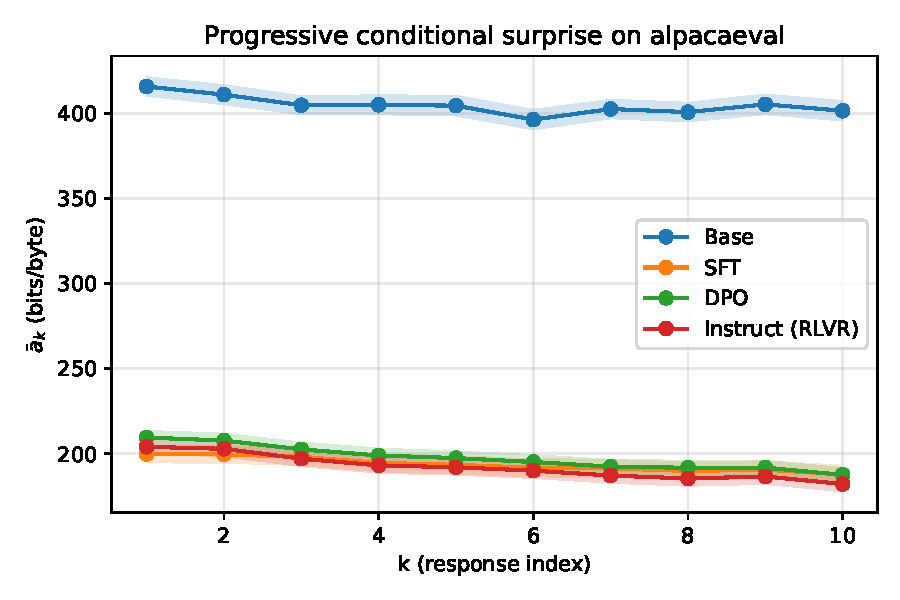
\includegraphics[width=\textwidth]{../figures/rlhf_experiment/ak_curves_overlay_alpacaeval.pdf}
    \caption{AlpacaEval $\bar{a}_k$ curves.}
\end{subfigure}\hfill
\begin{subfigure}[t]{0.48\textwidth}
    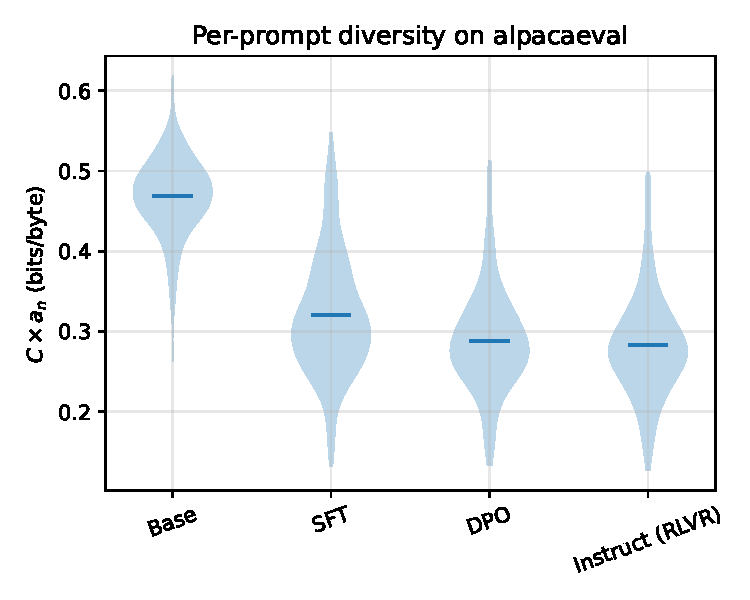
\includegraphics[width=\textwidth]{../figures/rlhf_experiment/per_prompt_D_violin_alpacaeval.pdf}
    \caption{Per-prompt $D_{Ca_n}$ by stage.}
\end{subfigure}
\caption{Progressive conditional surprise curves and per-prompt diversity distributions across the four OLMo-2-7B stages on AlpacaEval. Each later stage's $\bar{a}_k$ curve lies below the base curve at every $k \geq 2$; the per-prompt $D_{Ca_n}$ distribution shifts toward lower values as the pipeline advances.}
\label{fig:rlhf-ak-violin}
\end{figure*}
}{}

\IfFileExists{../figures/rlhf_experiment/metric_correlation_scatter_alpacaeval_lm.pdf}{%
\begin{figure*}[!htbp]
\centering
\begin{subfigure}[t]{\textwidth}
    \centering
    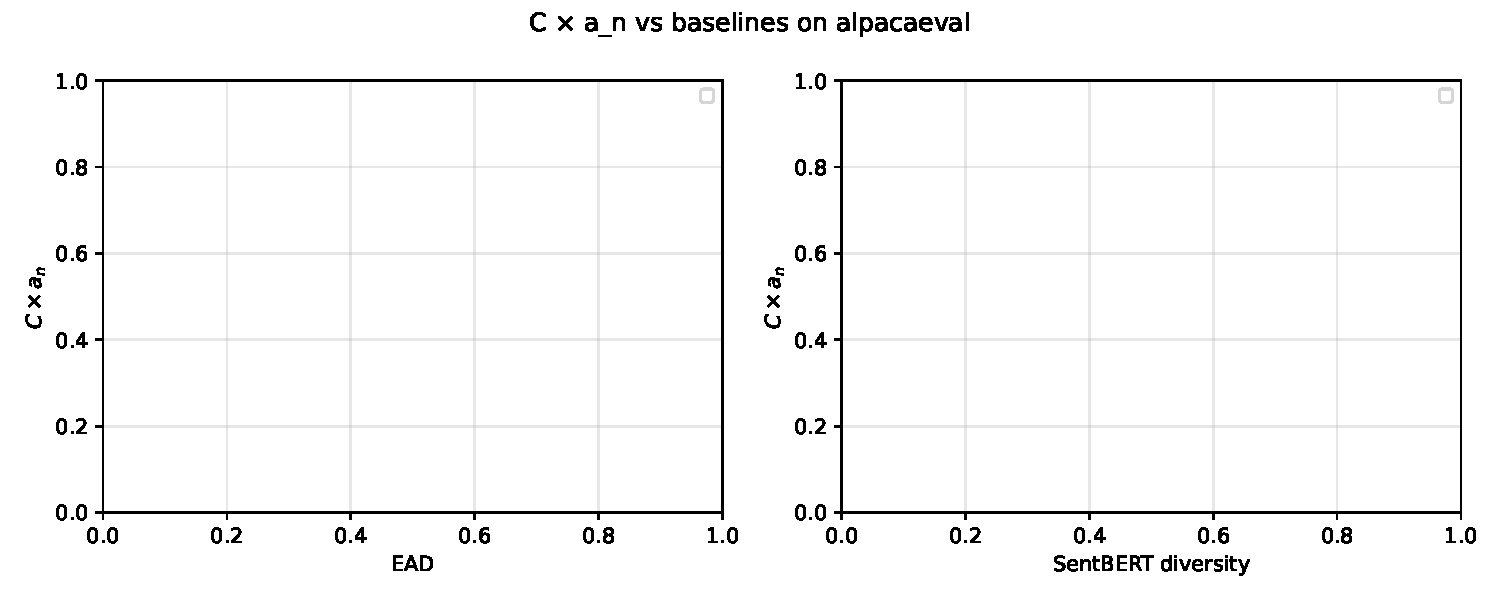
\includegraphics[width=0.85\textwidth]{../figures/rlhf_experiment/metric_correlation_scatter_alpacaeval_lm.pdf}
    \caption{AlpacaEval (length-matched, $n=\olmoLmAlpacaN$ prompts).}
\end{subfigure}\\[0.5em]
\begin{subfigure}[t]{\textwidth}
    \centering
    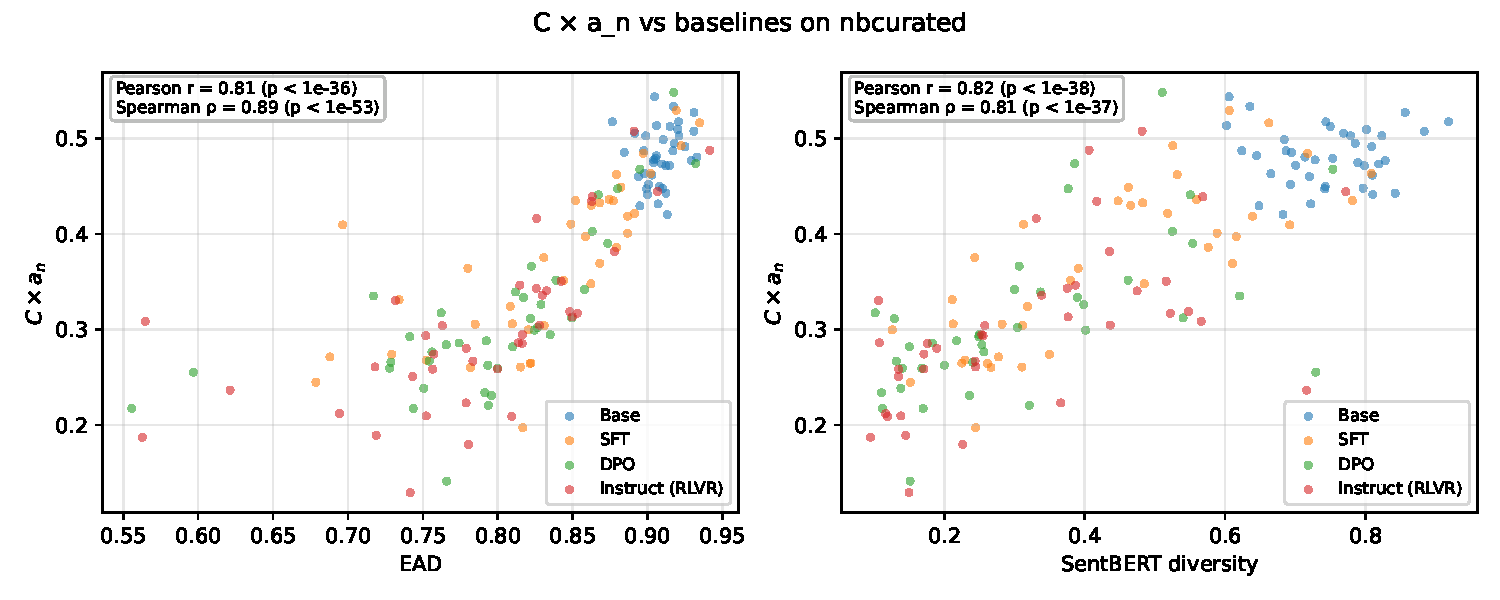
\includegraphics[width=0.85\textwidth]{../figures/rlhf_experiment/metric_correlation_scatter_nbcurated_lm.pdf}
    \caption{NoveltyBench curated (length-matched, $n=\olmoLmNbCuratedN$ prompts).}
\end{subfigure}
\caption{Per-prompt $D_{Ca_n}$ versus EAD (left subpanel) and SentBERT-similarity diversity (right subpanel), coloured by stage, on the length-matched subset of prompts. Length-matching truncates each (stage, prompt) tuple's responses to a common per-prompt byte budget so the per-byte conditional surprise that defines $a_n$ is not depressed by response length. Pearson $r$ and Spearman $\rho$ (two-sided $p$) are reported in each panel. The rank correlations are positive across both prompt sets and both baselines: $D_{Ca_n}$ tracks the same diversity-loss signal EAD and SentBERT detect, and the agreement is not an artefact of response length.}
\label{fig:rlhf-metric-scatter}
\end{figure*}
}{}

\paragraph{Discussion.} The monotone drop across all three pre-registered contrasts is consistent with the post-training-reduces-diversity findings of \citet{kirk2023rlhf,padmakumar2023writingreduces}, now measured by an information-theoretic metric that needs neither an embedding model nor a sentence similarity function.
Cross-metric agreement with EAD and SentBERT (Figure~\ref{fig:rlhf-metric-scatter}) confirms $D_{Ca_n}$ responds to the same signal lexical and semantic baselines detect.
The within-pipeline drop ($\sim$\olmoNbCuratedBaseDMean{} to \olmoNbCuratedInstructDMean{}, about 0.2 bits/byte across the four OLMo stages) is comparable in magnitude to the dispersion observed across an entire frontier instruct-model cluster on the same NoveltyBench-curated prompts; we defer the full cross-model table to a longer venue.

\paragraph{Released artefacts.} The \olmoAlpacaN$\,+\,$\olmoNbCuratedN{} prompts $\times$ 4 stages $\times$ $K{=}10$ generations are released as a public dataset (link withheld for double-blind review; an anonymous mirror is in supplementary materials).
To our knowledge this is the first public release of $K\!\ge\!10$ sampled responses across a paired SFT/DPO/RL pipeline, filling a gap that blocked direct diversity replication of \citet{kirk2023rlhf} (whose $K{=}16$ generations were logged only to a private W\&B project).

% --- macro fallbacks (only fire if the generated files are absent) ---
\providecommand{\olmoAlpacaN}{200}
\providecommand{\olmoNbCuratedN}{100}
\providecommand{\olmoAlpacaBaseDMean}{??}
\providecommand{\olmoAlpacaSftDMean}{??}
\providecommand{\olmoAlpacaDpoDMean}{??}
\providecommand{\olmoAlpacaInstructDMean}{??}
\providecommand{\olmoAlpacaHoneADz}{??}
\providecommand{\olmoAlpacaHoneAPbonf}{??}
\providecommand{\olmoAlpacaHoneBDz}{??}
\providecommand{\olmoAlpacaHoneBPbonf}{??}
\providecommand{\olmoAlpacaHoneCDz}{??}
\providecommand{\olmoAlpacaHoneCPbonf}{??}
\providecommand{\olmoAlpacaHpaDiff}{??}
\providecommand{\olmoAlpacaHpaDz}{??}
\providecommand{\olmoNbCuratedBaseDMean}{??}
\providecommand{\olmoNbCuratedSftDMean}{??}
\providecommand{\olmoNbCuratedDpoDMean}{??}
\providecommand{\olmoNbCuratedInstructDMean}{??}
\providecommand{\olmoNbCuratedHoneADz}{??}
\providecommand{\olmoNbCuratedHoneAPbonf}{??}
\providecommand{\olmoNbCuratedHoneBDz}{??}
\providecommand{\olmoNbCuratedHoneBPbonf}{??}
\providecommand{\olmoNbCuratedHoneCDz}{??}
\providecommand{\olmoNbCuratedHoneCPbonf}{??}

% Length-matched run macros (only the prompt counts are referenced here)
\providecommand{\olmoLmAlpacaN}{??}
\providecommand{\olmoLmNbCuratedN}{??}

% Cross-model comparison table macros
\providecommand{\crossModelOlmoBase}{??}
\providecommand{\crossModelOlmoSft}{??}
\providecommand{\crossModelOlmoDpo}{??}
\providecommand{\crossModelOlmoInstruct}{??}
\providecommand{\crossModelQwenFourB}{??}
\providecommand{\crossModelQwenEightB}{??}
\providecommand{\crossModelQwenTwoThreeFiveB}{??}
\providecommand{\crossModelLlamaThreeThreeSeventyB}{??}
\providecommand{\crossModelGptFiveNano}{??}
\providecommand{\crossModelGptFive}{??}
\providecommand{\crossModelClaudeSonnetFourFive}{??}

\section{Limitations}\label{sec:limitations}

We collect the main limitations of the framework and of our $D = C \times a_n$ choice in one place so readers can calibrate how strongly to update on the results above.
Several points below recap caveats already made in their natural context and cross-reference those for detail.

\paragraph{Measurement is relative to $\theta$'s perception.}
The metric evaluates diversity \emph{as perceived by the base model $\theta$}: if $\pi$'s outputs differ only in ways $\theta$ cannot distinguish from context, the metric underestimates diversity (Section~\ref{sec:motivation}, ``Important caveat'').

\paragraph{Cross-mode learning is model-dependent.}
The off-diagonal sign of the pairwise surprise-reduction matrix changes with $\theta$'s scale (Section~\ref{sec:cross-mode-learning}): $a_k$ curves for the same response set are not directly comparable across different choices of $\theta$.

\paragraph{Metric selection saw the full Tevet benchmark.}
We chose $C \times a_n$ (rather than alternative summaries such as $C \times E$; Appendix~\ref{app:excess-entropy}) after observing its performance on the full Tevet diversity-eval benchmark, without holding out a validation split.
The Tevet numbers in Section~\ref{sec:tevet} may therefore be optimistically biased: the scalar form was selected with visibility into those results.
The OLMo-2-7B post-training experiment (Section~\ref{sec:rlhf-experiment}) was scored after the metric form was fixed and provides independent validation; the synthetic mode-count experiments (Section~\ref{sec:mode-count-scaling}) informally influenced the choice (had they failed, we would likely have revised the metric) and so are not strictly independent.

\paragraph{External benchmark performance trails the strongest baseline.}
On Tevet and Berant's diversity-eval benchmark, $C \times a_n$ trails SentBERT by \tevetCxAnVsSentBertOCAMinPct\%--\tevetCxAnVsSentBertOCAMaxPct\% OCA across the nine binary tasks (Section~\ref{sec:tevet}); scaling the base model to Qwen3-30B-A3B-Base did not close the gap (Appendix~\ref{app:qwen3-comparison}).
We position $C \times a_n$ as a principled complement to embedding-based metrics, not a replacement.

\paragraph{Prompt format is fixed.}
We use a neutral ``Response A: \ldots, Response B: \ldots'' template throughout and have not attempted prompt optimisation; targeted prompt engineering could plausibly improve discriminative power, especially for larger base models (Section~\ref{sec:exp-discussion}).

\paragraph{Length-matching drops short-response prompts.}
$C$ and $a_n$ are both per-byte quantities, but neither is invariant to response length: in a causal LM, longer responses give $\theta$ more within-response context to predict later tokens, lowering per-byte surprise.
For the OLMo-2-7B experiment (Section~\ref{sec:rlhf-experiment}) raw response length is not monotone across stages, so we score the length-matched subset as the headline analysis: every response in a (stage, prompt) tuple is truncated to a common per-prompt UTF-8 byte length (the minimum across all 40 responses) before scoring.
$111/300$ prompts had a per-prompt common length below 50 bytes — driven by the base model on AlpacaEval (no instruction-following prior) and by SFT on NB-curated short-answer prompts — and were dropped because length-matching them would compare essentially-empty fragments.
The headline numbers therefore condition on the $150/200$ AlpacaEval and $39/100$ NB-curated prompts where length-matching is well-defined; the dropped prompts are themselves a stage-specific behavioural signal we are not measuring here.
We also verified that the monotone $D$ drop holds on the un-truncated $200+100$ prompt sets, with all three pre-registered H1 contrasts remaining Bonferroni-significant at $p<10^{-13}$ on both prompt sets.
Full numbers and reproduction commands are in \path{investigations/length_matched_rlhf/VERDICT.md}.

\paragraph{$D = C \times a_n$ is a pragmatic choice, not a theoretically derived one.}
The product form was selected because it captures the properties we wanted a diversity score to have (residual surprise remains after the base model has seen previous responses, low-coherence outputs are penalised, and the result stays on a bits-per-byte scale), not because it is derived from an axiomatic information-theoretic setup.
Other scalars respecting the same constraints (weighted integrals of $a_k - a_\infty$, slope-based scores, or coherence applied at a different point on the curve) could equally be defended (see ``The framework admits other metrics'' in Section~\ref{sec:exp-discussion}).
We adopt $D_{Ca_n}$ because it is interpretable and works empirically across our validation regimes, not because it is uniquely correct.
We invite other researchers to build on this work to develop other formulas that characterize the $a_k$ curve in meaningful ways.
\section{Conclusion}\label{sec:conclusion}

$D_{Ca_n} = C \times a_n$ is an information-theoretic diversity metric that uses a base model's in-context learning to detect similarities between arbitrary numbers of responses in a single forward pass.
It requires no embedding model, no reference corpus, no human labels, and no special-purpose training.
The same pipeline scores AI samples and human-written sets.
On Tevet and Berant's human-grounded benchmark it is near the level of the strongest sentence-embedding baseline.
On the OLMo-2-7B post-training pipeline it drops across the base $\to$ SFT $\to$ DPO/RLVR stages, tracking the diversity loss attributed to RLHF-style training.


% Acknowledgements deferred to arXiv v2 (pending contributor consent).
% Text kept in sections/acknowledgements_workshop.tex but intentionally NOT
% \input here for v1; re-add the \input line below to include it in v2.

\section*{Impact Statement}

This paper presents work which may be used in evaluation pipelines that select for more capable AI systems.
We view the prospect of increasingly capable future AI as one of unclear positive or negative net impact.
This work may also contribute to the automation of human creative roles.
We publish it in the hope that better understanding of machine-generated diversity will contribute to better evaluation and oversight, and that these benefits outweigh the risks.


\bibliography{refs}
\bibliographystyle{icml2026}

\newpage
\appendix
% Material trimmed from the 4--8 page main body lives here. Reviewers may skip.
\section{Practical Considerations}\label{sec:practical}

\subsection{Formatting the Conditioning Context}

Computing $\theta(r_k \mid r_{<k}, p)$ requires feeding $\theta$ a context containing the prompt and previous responses.
The formatting choice affects results.
We recommend using a base (non-instruction-tuned) model as $\theta$ and formatting as:

\begin{verbatim}
    [prompt p]

    Response A: [r_1]

    Response B: [r_2]

    Response C: [r_3]
\end{verbatim}

This leverages the base model's in-context learning to treat the responses as parallel completions.
An instruction-tuned model might instead interpret previous responses as conversation turns, confounding the measurement.

\paragraph{Base vs.\ instruction-tuned models.} We use a base (non-instruction-tuned) model as $\theta$ for two reasons.
First, an instruction-tuned model has had its output distribution shaped by RLHF or similar procedures, so using one as $\theta$ reintroduces the kind of distributional bias we seek to avoid.
Second, an instruction-tuned $\theta$ may assign systematically different probabilities to text that follows or violates its alignment training, introducing a confound between coherence-as-fluency and coherence-as-alignment that the metric should not conflate.
Modern base models already exhibit strong in-context learning from pretraining alone, so this choice does not sacrifice ICL capability.
Optimizing the prompt format to maximally elicit in-context learning from $\theta$ is an interesting direction but out of scope for this paper; we use the neutral ``Response A/B/C'' template throughout.

\subsection{Computational Cost}\label{sec:cost}

Because $\theta$ is a causal language model, the full $a_k$ curve can be computed from a \textbf{single forward pass}.
Concatenate the prompt and all responses into one sequence:

\begin{verbatim}
    [prompt p] Response A: [r_1] Response B: [r_2] ... Response N: [r_n]
\end{verbatim}

The forward pass produces the log-probability of every token conditioned on all preceding tokens.
The tokens belonging to $r_k$ are conditioned on exactly $p, r_1, \ldots, r_{k-1}$ (plus formatting), which is the conditioning required for $a_k$.
Partitioning the output log-probabilities by response boundary and summing within each partition yields all $n$ values of $a_k$ simultaneously.
The cost is a single forward pass over the full concatenation, with FLOPs scaling as $O((|p| + n\bar{L}_{\mathrm{tok}})^2)$ from causal attention, where $\bar{L}_{\mathrm{tok}}$ is the average response length in tokens.

The coherence term $C$ and spread $\sigma_\ell$ additionally require the \emph{unconditional} per-byte cross-entropies $h_\theta(r_i \mid p)$ for each response.
These cannot be extracted from the concatenated pass, since in that pass $r_i$ for $i > 1$ is conditioned on all prior responses.
Computing them requires $n$ independent forward passes, each over the short context $(p, r_i)$.
These passes are embarrassingly parallel and batchable.

In summary:
\begin{itemize}[nosep]
    \item $a_k$ curve: 1 forward pass per permutation (long context).
    \item $C$ and $\sigma_\ell$: $n$ forward passes (short contexts, batchable).
\end{itemize}

\subsection{Dependence on Sample Ordering}\label{sec:ordering}

The $a_k$ values depend on the ordering of $\{r_i\}$.
Since raw $a_k$ is in total bits, responses of different lengths produce different values even at the same per-byte rate, making a single ordering's curve jagged.
Averaging over random permutations removes this length effect: each position averages over all responses, so the curve reflects only how $\theta$'s predictions improve with more context.
We recommend averaging over a moderately large number of random permutations; Section~\ref{sec:practical-findings} provides empirical evidence that $\geq 50$ permutations are needed for reliable rankings.

Per-response normalization by byte count must be performed \emph{before} averaging across permutations, since the byte count depends on which response lands at each position.
Concretely, the per-byte curve is a mean of per-permutation rates,
\begin{equation}\label{eq:akbar-mor}
    \bar{a}_k = \frac{1}{|\Sigma|}\sum_{\sigma \in \Sigma} \frac{a_k^{\sigma}}{\|r_{\sigma(k)}\|},
\end{equation}
not a ratio of permutation-averaged bits to permutation-averaged byte counts (which would degenerate, after enough permutations, into the total-bits curve rescaled by the mean response length).

\subsection{Choice of $n$}

The diversity score depends on $n$ through the estimate $a_n \approx a_\infty$.
We recommend choosing $n$ large enough that $a_n$ has approximately stabilized (i.e., the curve has reached its floor), and fixing $n$ across all comparisons for consistency.
A practical choice is $n = 10$--20, which suffices for policies where $\theta$'s learning stabilizes within this range.

\paragraph{Detectable mode weight.} Modes with weight $w \lesssim 1/n$ will rarely appear in the sample, and even when they do, $\theta$ has insufficient examples to learn the pattern.
As a rough guide, modes with weight below $1/n$ are invisible to the metric.
For $n = 15$, this means modes contributing less than $\sim$7\% of the probability mass are unlikely to be captured.
If rare modes are of interest (e.g., when evaluating whether an intervention eliminates low-frequency behaviors), $n$ should be increased accordingly, subject to the context-length constraints discussed above.

%%%%%%%%%%%%%%%%%%%%%%%%%%%%%%%%%%%%%%%%%%%%%%%%%%%%%%%%%%%%%%%%%%%%%%%%
%% SECTION 8: EXPERIMENTS
%%%%%%%%%%%%%%%%%%%%%%%%%%%%%%%%%%%%%%%%%%%%%%%%%%%%%%%%%%%%%%%%%%%%%%%%

\section{Experiments}\label{sec:experiments}

\subsection{Experimental Setup}\label{sec:exp-setup}

We evaluate the metric primarily using Qwen2.5-3B (3B parameters, 128K-token context window) \citep{yang2024qwen25}, with GPT-2 (124M parameters, 1024-token context window) \citep{radford2019language} as a smaller-model comparison point for scenario validation.
Qwen2.5-3B is used for mode-count scaling, cross-mode learning, and external validation (Sections~\ref{sec:mode-count-scaling}, \ref{sec:cross-mode-learning}, \ref{sec:tevet}).
The cross-model scaling study (Section~\ref{sec:exp-discussion}) additionally uses the full Llama 3 family for comparison.

All $a_k$ curves are computed using single-pass forward computation (Section~\ref{sec:cost}).
Unless otherwise noted, we use 100 permutations for scenario validation and 50 permutations for larger-scale experiments.
Responses are formatted as described in Section~\ref{sec:cost}.
All code is publicly available.\footnote{\url{https://github.com/AMindToThink/icl-diversity}}


\subsection{Scenario Validation}\label{sec:scenario-validation}

We construct five synthetic scenarios with known diversity structure:
\begin{enumerate}[nosep]
    \item \textbf{Pure noise}: Random word salad with no learnable structure.
    \item \textbf{Multi-incoherent}: Responses from 5 distinct modes, each internally incoherent (scrambled words within a template).
    \item \textbf{Multi-mode}: Responses from 5 distinct modes, each internally coherent (e.g., recipe, poem, code).
    \item \textbf{One-mode}: All responses from a single coherent mode (paraphrases of the same content).
    \item \textbf{Mixed}: A mixture of coherent and incoherent responses.
\end{enumerate}

Each scenario contains 10 responses per prompt, 5 prompts per scenario, with 100 permutations and seed 42.

\begin{table}[t]
\centering
\caption{Scenario validation metrics (mean across 5 prompts, 100 permutations, $n=10$ responses, per-byte).
We report several candidate scalars: unconditional surprise $a_1$, the asymptotic floor $a_n$, coherence $C$, our recommended score $D_{Ca_n} = C \times a_n$ (\textbf{bold}), the excess entropy $E$ (Appendix~\ref{app:excess-entropy}), $C \times E$, and the coherence spread $\sigma_\ell$. $D_{Ca_n}$ correctly ranks multi-mode above one-mode and suppresses incoherent scenarios via $C$.
Both $E$ and $C \times E$ go negative for the mixed scenario on GPT-2.}
\label{tab:scenarios}
\small
% Generated by: scripts/generate_scenario_table.py
% Data sources: results/scenario_metrics_v2_100perm.json
%               results/scenario_metrics_v2_qwen_100perm.json
\begin{tabular}{@{}l rrrrrrr rrrrrrr@{}}
\toprule
& \multicolumn{7}{c}{\textbf{GPT-2 (124M)}} & \multicolumn{7}{c}{\textbf{Qwen2.5-32B}} \\
\cmidrule(lr){2-8} \cmidrule(lr){9-15}
Scenario & $a_1$ & $a_n$ & $C$ & $\mathbf{D_{a_\infty}}$ & $E$ & $C\!\times\!E$ & $\sigma_\ell$ & $a_1$ & $a_n$ & $C$ & $\mathbf{D_{a_\infty}}$ & $E$ & $C\!\times\!E$ & $\sigma_\ell$ \\
\midrule
Pure noise & 7.32 & 6.84 & 0.006 & \textbf{0.04} & 0.55 & 0.003 & 0.20 & 6.85 & 6.56 & 0.009 & \textbf{0.06} & 0.44 & 0.004 & 0.09 \\
Multi-incoher. & 2.99 & 1.66 & 0.12 & \textbf{0.20} & 5.64 & 0.68 & 0.51 & 1.93 & 1.19 & 0.27 & \textbf{0.33} & 2.42 & 0.66 & 0.84 \\
Multi-mode & 1.02 & 0.53 & 0.50 & \textbf{0.26} & 1.55 & 0.75 & 0.08 & 0.71 & 0.26 & 0.62 & \textbf{0.16} & 1.21 & 0.74 & 0.09 \\
One-mode & 1.02 & 0.22 & 0.50 & \textbf{0.11} & 1.24 & 0.61 & 0.06 & 0.74 & 0.15 & 0.60 & \textbf{0.09} & 0.85 & 0.51 & 0.08 \\
Mixed & 1.62 & 1.71 & 0.29 & \textbf{0.49} & $-$1.27 & $-$0.34 & 1.12 & 0.77 & 0.56 & 0.57 & \textbf{0.32} & 0.69 & 0.39 & 0.47 \\
\bottomrule
\end{tabular}

\end{table}

\paragraph{Results.} Table~\ref{tab:scenarios} summarizes the metrics.
Figure~\ref{fig:scenario-curves} shows the $a_k$ curves for all scenarios.

\begin{figure}[t]
\centering

\includegraphics[width=\textwidth,height=0.4\textheight,keepaspectratio]{comparison_v3/comparison_ak_curves_all.png}
\caption{Progressive conditional surprise curves ($a_k$, per-byte) for all five scenarios, comparing GPT-2 (top row) and Qwen2.5-3B (bottom row).
In each panel, faint colored curves are individual permutations (100 per prompt), medium colored curves are per-prompt averages, and the bold black curve is the mean across prompts.
Pure noise curves are flat (no learnable structure); multi-mode curves show progressive decline; one-mode curves decline steeply then flatten.}
\label{fig:scenario-curves}
\end{figure}

The coherence term $C$ correctly separates coherent from incoherent scenarios: $C \approx 0.5$--$0.6$ for multi-mode and one-mode, $C \approx 0.1$--$0.3$ for multi-incoherent, and $C \approx 0.01$ for pure noise.
The coherence spread $\sigma_\ell$ discriminates mixed from pure scenarios: $\sigma_\ell > 1.0$ for mixed (GPT-2), reflecting the within-set heterogeneity between coherent and incoherent responses.

$C$ consistently improves with model strength (Qwen2.5-3B assigns higher coherence to genuinely coherent text than GPT-2). $D_{Ca_n}$ correctly ranks multi-mode above one-mode on both models, and suppresses pure noise and multi-incoherent via the $C$ factor.


\subsection{Mode Count Scaling}\label{sec:mode-count-scaling}

To test whether the metric reflects the number of distinct modes, we construct response sets with $m \in \{1, \ldots, \modeCountMMax\}$ modes drawn from a pool of \modeCountPoolSize{} format-based generators (haiku, code, recipe, legal disclaimer, etc.), all responding to the same prompt (``Write a short piece about rain'').
For Qwen2.5-3B: $n=\modeCountNResponses$ responses, \modeCountNDraws{} random draws of mode assignments, averaged over permutations.

\begin{figure}[!htbp]
\centering

\includegraphics[width=\columnwidth]{mode_count/qwen2.5-3b/ak_curves_overlay.png}
\caption{Mode count scaling on Qwen2.5-3B ($n=\modeCountNResponses$, \modeCountNDraws{} draws).
The $a_k$ curves fan out with increasing $m$: higher floors, slower convergence.
All curves are exponential (no sigmoidal plateau), even at $m=\modeCountMMax$, due to cross-mode learning (Section~\ref{sec:cross-mode-learning}).
Shaded bands around each curve are $\pm 1$ standard error of the mean across the \modeCountNDraws{} random draws of mode assignments (i.e., the across-draw standard deviation divided by $\sqrt{\modeCountNDraws}$); they are narrow because averaging over \modeCountNDraws{} draws sharply reduces the across-draw spread.}
\label{fig:mode-count}
\end{figure}

\paragraph{Key findings.} Figure~\ref{fig:mode-count} shows the $a_k$ curves.
$a_n$ increases monotonically with $m$ (\modeCountAnMone{} bits at $m=1$ to \modeCountAnMten{} bits at $m=10$; see Table~\ref{tab:mode-count}), reflecting that with more modes there are fewer same-mode repetitions within $n$ responses, so each response remains more surprising even after $\theta$ has seen the others.
This is exactly the behavior $D_{Ca_n} = C \times a_n$ needs: $a_n$ tracks mode count directly.
All curves are purely exponential (no sigmoidal plateau), even at $m=10$; Section~\ref{sec:cross-mode-learning} investigates why.
For a detailed comparison of the excess-entropy-based scores on this data, including the sigmoid fit parameters and the non-monotonicity of $\hat{E}_n$, see Appendix~\ref{app:excess-entropy}.


\subsection{Cross-Mode Learning and Curve Shape}\label{sec:cross-mode-learning}

The paper predicts that at high $m$, the $a_k$ curve should be sigmoidal: an initial plateau (early responses come from different modes and are uninformative about each other), followed by decline once mode repetitions accumulate.
GPT-2 shows this pattern at $m=10$.
Qwen2.5-3B does not: it shows immediate exponential decay at all $m$.
This section investigates the discrepancy through systematic pairwise analysis.

\paragraph{Pairwise cross-mode surprise matrix.} For 15 modes, we compute a $15 \times 15$ matrix $M_{ij}$: the surprise reduction (in bits) when a response from mode $j$ is in the context and mode $i$ is the target.
Diagonal entries measure same-mode learning; off-diagonal entries measure cross-mode information transfer.
Each entry averages over 5 context--target samples (using different samples for context and target to avoid self-prediction inflation).

\begin{figure*}[p]
\centering
\begin{subfigure}{\textwidth}
    \centering
    
\includegraphics[width=\textwidth]{pairwise_matrix_heatmap.png}
    \caption{Qwen2.5-3B: positive off-diagonal.}
    \label{fig:pairwise-qwen}
\end{subfigure}

\vspace{1.5em}

\begin{subfigure}{\textwidth}
    \centering
    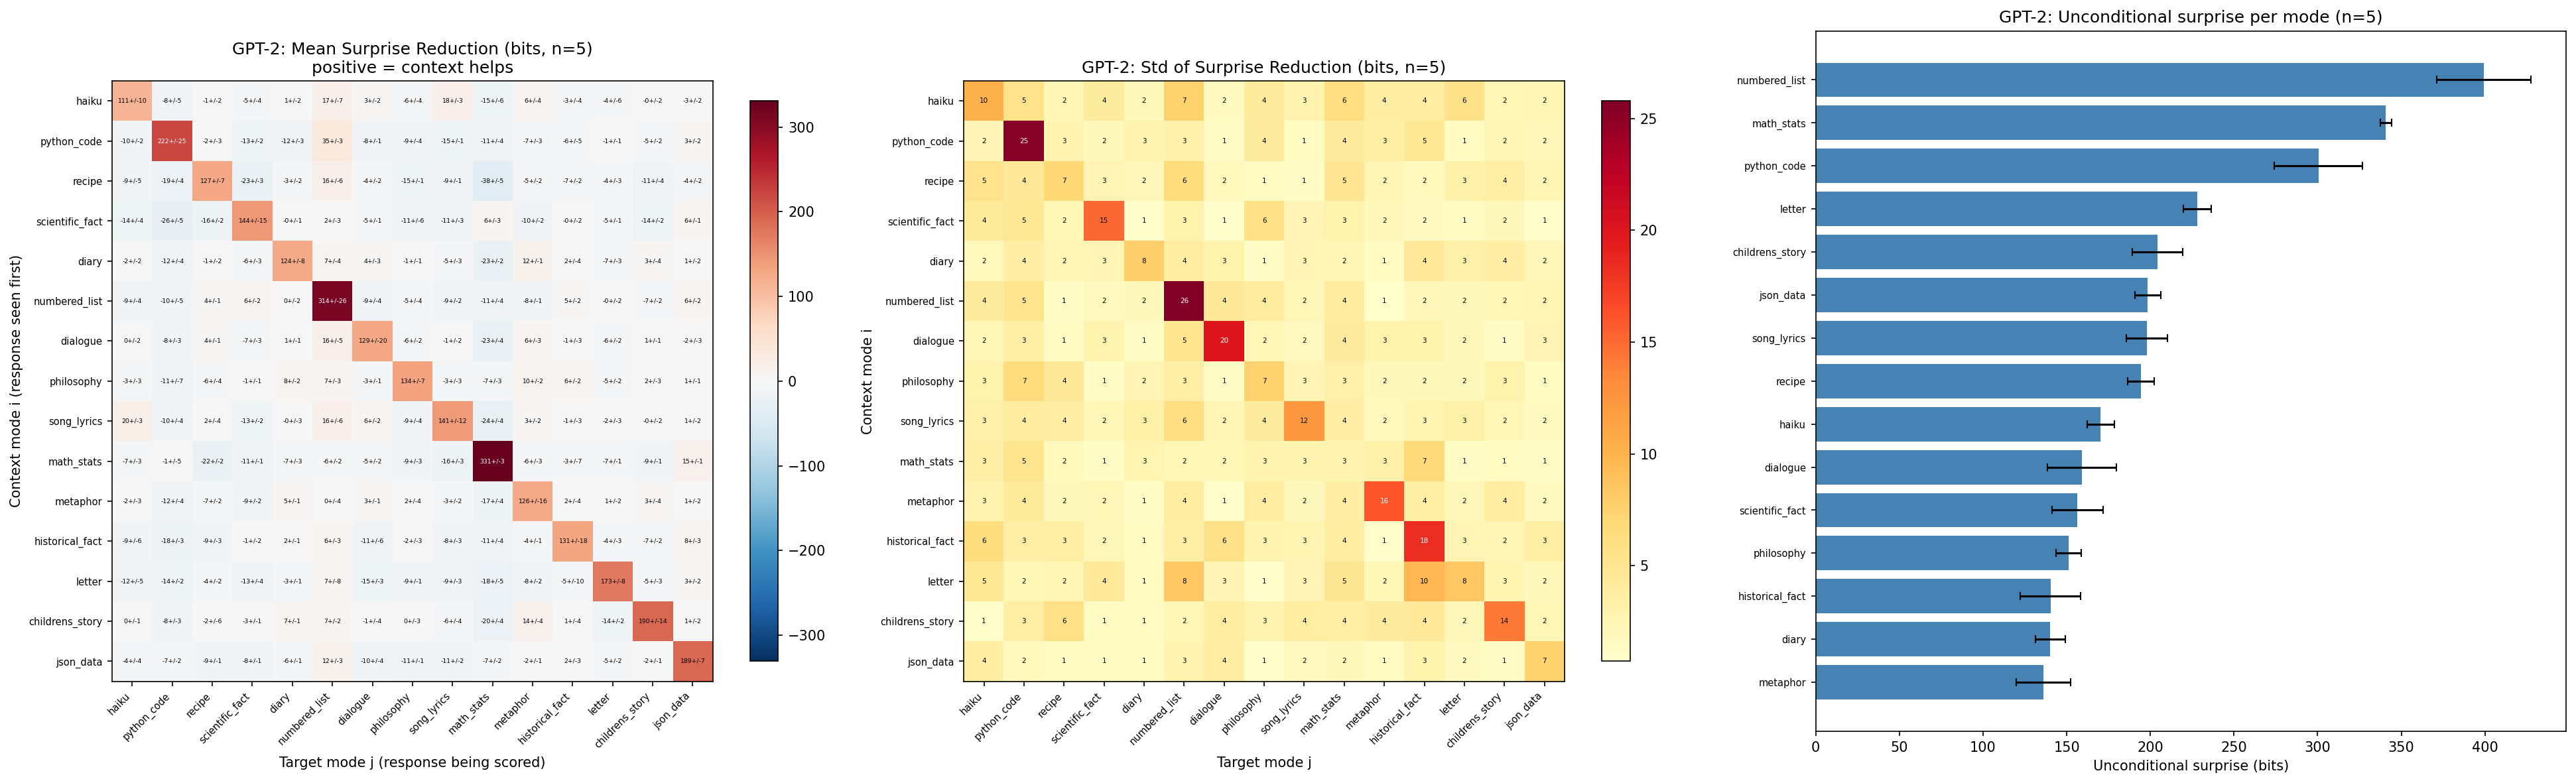
\includegraphics[width=\textwidth]{gpt2/pairwise_matrix_heatmap.png}
    \caption{GPT-2: negative off-diagonal.}
    \label{fig:pairwise-gpt2}
\end{subfigure}
\caption{Pairwise cross-mode surprise reduction matrices.
Each cell $(i,j)$ shows how many bits of surprise reduction mode $i$ (target) receives from seeing mode $j$ (context).
Qwen shows diagonal dominance with pervasive positive off-diagonal (\crossmodeQwenOffMean{} bits mean); GPT-2 shows diagonal dominance with negative off-diagonal (\crossmodeGPTOffMean{} bits mean).}
\label{fig:pairwise-matrices}
\end{figure*}

\paragraph{Results.} (Cell standard deviations are the mean within-cell sampling std across the \crossmodeNumModes{} diagonal or \crossmodeNumOffPairs{} off-diagonal matrix cells, each estimated from 5 context-target sample pairs.)
\begin{itemize}[nosep]
    \item \textbf{Qwen2.5-3B}: diagonal mean = $\crossmodeQwenDiagMean \pm \crossmodeQwenDiagStd$ bits, off-diagonal mean = $\crossmodeQwenOffMean \pm \crossmodeQwenOffStd$ bits, \crossmodeQwenOffPctPos\% of off-diagonal entries positive.
    \item \textbf{GPT-2}: diagonal mean = $\crossmodeGPTDiagMean \pm \crossmodeGPTDiagStd$ bits, off-diagonal mean = $\crossmodeGPTOffMean$ bits, only \crossmodeGPTOffPctPos\% of off-diagonal entries positive.
\end{itemize}

The sign of the off-diagonal determines the curve shape (Figure~\ref{fig:pairwise-matrices}):
\begin{itemize}[nosep]
    \item \textbf{Positive off-diagonal (Qwen)}: Every response helps predict every other response through format calibration and topic priming.
The $a_k$ curve drops from position 1, producing exponential decay.
    \item \textbf{Negative off-diagonal (GPT-2)}: Cross-mode responses actively interfere with predictions.
At $m=10$, the expected first-step net drop under the additive independent-mode model is only $\crossmodeGPTFirstStepDrop$ bits (the \crossmodeGPTDiagGainMten{}-bit diagonal gain from the $1/m$ same-mode chance is largely offset by the $\crossmodeGPTCrossDamageMten$-bit cross-mode damage from the $(m{-}1)/m$ different-mode chance), producing a flat plateau until same-mode repetitions accumulate, the predicted sigmoid.
\end{itemize}

\paragraph{From pairwise matrix to full curve.} The sign-of-off-diagonal calculation above recovers the qualitative shape difference between Qwen and GPT-2 from pairwise measurements alone.
Extending to the full $a_k$ curve at $m>1$ requires modeling information overlap across repeated encounters --- structure that pairwise (single-encounter) measurements do not capture.
Additive and fractional decompositions of the pairwise matrix both fail in instructive ways but neither is load-bearing for our thesis; we omit the details.

\paragraph{Pairwise asymmetry.} The mean absolute asymmetry $|M_{ij} - M_{ji}|$ is \crossmodeAsymmetryMean{} bits ($\crossmodeAsymmetryRatio\times$ the off-diagonal mean), falsifying the hypothesis that pairwise surprise reduction is symmetric (Figure~\ref{fig:pairwise-symmetry}).
This reflects different mechanisms: technical/structured modes (code, JSON, math) are highly informative as context (format calibration) but do not benefit proportionally from other modes' context.

\begin{figure*}[t]
\centering

\includegraphics[width=0.5\textwidth]{pairwise_symmetry.png}
\caption{Pairwise symmetry scatter for Qwen2.5-3B: each point is one $(i,j)$ pair, plotting $M_{ij}$ vs.\ $M_{ji}$.
Under symmetric mutual information, points would lie on $y = x$.
The best-fit slope is \scalingSymSlopeQwen{} ($R^2 = \scalingSymRsqQwen$), and many pairs have opposite signs: mode $i$ can reduce surprise for mode $j$ while $j$ \emph{increases} surprise for $i$.}
\label{fig:pairwise-symmetry}
\end{figure*}

\paragraph{Connections to information-theoretic properties.} Two information-theoretic properties are relevant to interpreting the pairwise matrix:

\begin{enumerate}[nosep]
    \item \textbf{Non-negative conditioning} ($H(X) \geq H(X \mid Y)$): Under the true distribution, conditioning can never increase entropy on average.
For cross-entropies this is not guaranteed (the KL term can increase), but a well-calibrated $\theta$ should show mostly non-negative off-diagonal entries.
    \item \textbf{Symmetry of mutual information} ($I(X;Y) = I(Y;X)$): Under the true joint, row means (how informative mode $i$ is as context) should correlate with column means (how much mode $i$ benefits from context).
\end{enumerate}

\begin{figure*}[t]
\centering
\begin{subfigure}[t]{0.48\textwidth}
    
\includegraphics[width=\textwidth]{pairwise_row_vs_col.png}
    \caption{Qwen2.5-3B: slope = \scalingRCSlopeQwen{}, $R^2 = \scalingRCRsqQwen$.}
    \label{fig:rowcol-qwen}
\end{subfigure}
\hfill
\begin{subfigure}[t]{0.48\textwidth}
    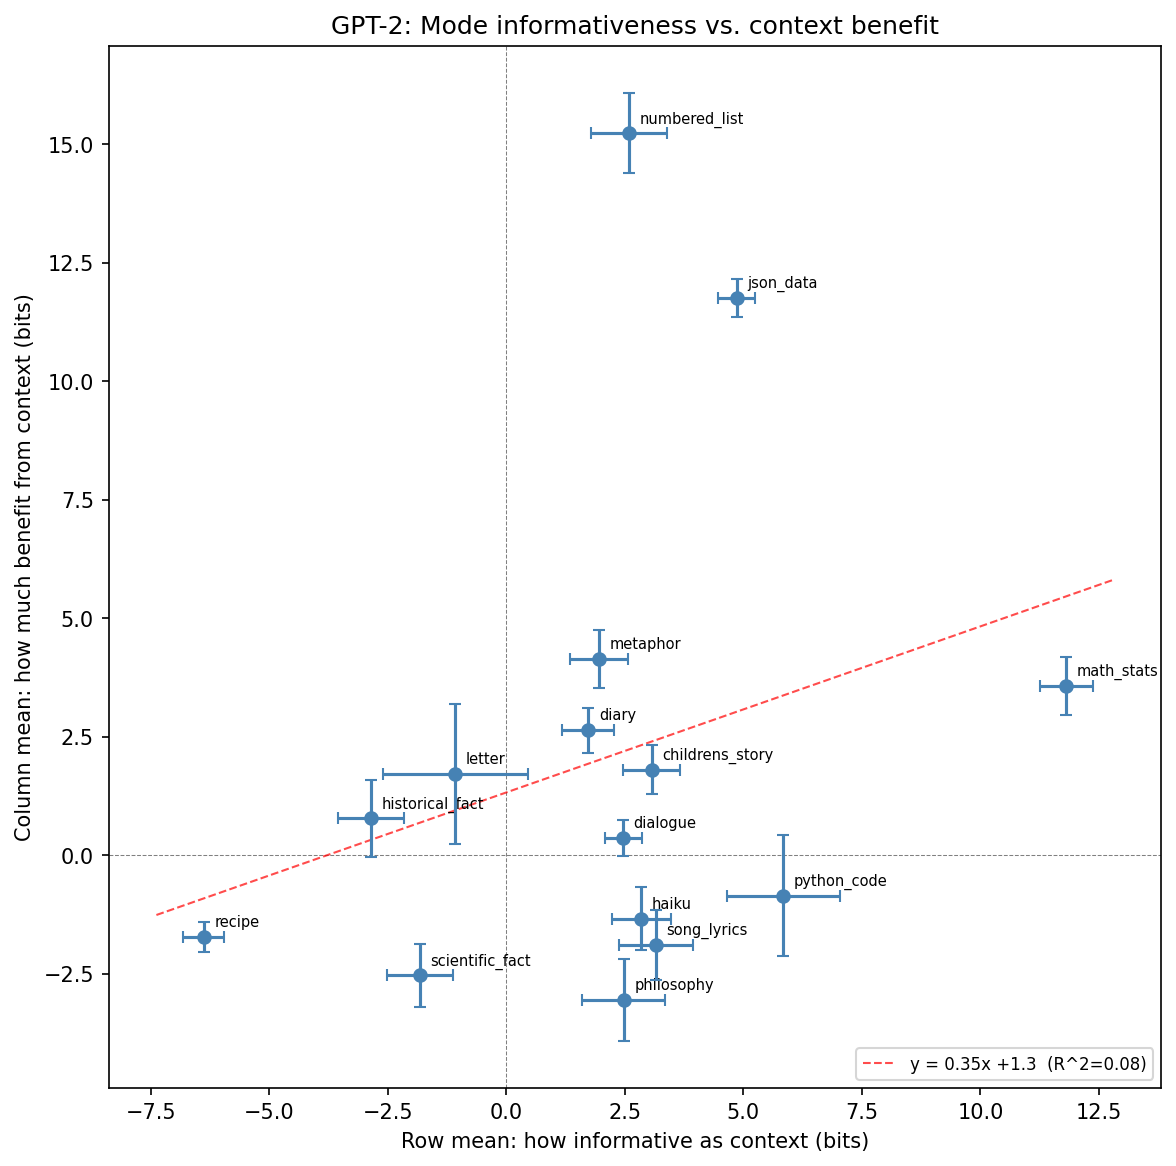
\includegraphics[width=\textwidth]{gpt2/pairwise_row_vs_col.png}
    \caption{GPT-2: slope = \scalingRCSlopeGPT{}, $R^2 = \scalingRCRsqGPT$.}
    \label{fig:rowcol-gpt2}
\end{subfigure}
\caption{Row mean (how informative as context) vs.\ column mean (how much benefit from context) for each mode.
Qwen shows tighter correlation closer to the identity, consistent with approximate symmetry of mutual information.
GPT-2 shows widespread violations of non-negative conditioning (modes in the negative-row-mean region).}
\label{fig:row-vs-col}
\end{figure*}

Figure~\ref{fig:row-vs-col} compares the two models.
Qwen shows a tighter row--column relationship (slope = \scalingRCSlopeQwen{}, $R^2 = \scalingRCRsqQwen$) with only \crossmodeQwenNegColCount{} of \crossmodeNumModes{} modes having a negative column mean.
GPT-2 shows widespread violations of non-negative conditioning (\crossmodeGPTNegColCount{} modes with negative column means) and a barely-existent row--column relationship (slope = \scalingRCSlopeGPT{}, $R^2 = \scalingRCRsqGPT$).
With only two base models tested, we have suggestive but not conclusive evidence that stronger models better satisfy these information-theoretic properties.

\paragraph{Token-level mechanisms.} Per-token attribution analysis reveals two mechanisms for cross-mode surprise reduction:
\begin{itemize}[nosep]
    \item \textbf{Format calibration} (front-loaded): Seeing any structured response recalibrates the model's expectations about what follows ``Response B:''.
This effect concentrates in the first few tokens of the target response; the per-pair magnitude varies widely (positive for most cross-mode pairs, negative when the context format actively conflicts with the target).
    \item \textbf{Topic/vocabulary priming} (distributed): All responses are about rain, so rain-related vocabulary gets primed cross-mode.
This contribution is spread across the target response rather than concentrated at the start.
\end{itemize}

\paragraph{Discussion.} The paper's sigmoid prediction assumes modes are approximately independent.
For capable models, this fails: cross-mode learning (format calibration, topic priming) creates positive information transfer between distinct modes.
The comparison between GPT-2 and Qwen is suggestive: the stronger model shows behavior closer to information-theoretic ideals.
If this pattern holds across more models, it would mean the metric's theoretical properties are better satisfied as $\theta$'s ICL capability improves, but confirming this requires testing additional base models of varying sizes.


% arXiv v2 candidate (drafted 2026-08; NOT in camera-ready v1): structural
% redundancy invisible to SentBERT / distinct-n. Uncomment for v2.
% % arXiv v2 draft section (NOT in the camera-ready workshop build; the \input
% line in main_icml_workshop.tex is commented out until v2).
% Experiments: reports/TEMPLATE_VS_SENTBERT.md and
% reports/POS_PATTERN_VS_BASELINES.md.
% Every inline number is a macro from results/tables/paper_macros.tex
% (template_frames_macros / pos_pattern_macros in scripts/build_paper_macros.py).

\subsection{Structural Redundancy Invisible to Embedding and $n$-gram Baselines}\label{sec:structural-redundancy}

Baseline diversity metrics each detect one family of similarity: embedding metrics score shared meaning \citep{reimers2019sbert}, and $n$-gram metrics score shared surface strings \citep{li2016diversity,zhu2018texygen}.
In-context learning has no such restriction: $\theta$ can pick up any regularity it can learn from context, including \emph{structural} redundancy, where responses share a sentence pattern while overlapping in neither vocabulary nor meaning.
We test this contrast on two synthetic generator families, scoring with the same Qwen2.5-3B base model \citep{yang2024qwen25} as our main experiments and computing baselines with the conventions of \citet{tevet2020evaluating}.
Both experiments use fully independent draws per condition with one random response ordering each, so statistical power comes from across-draw variation rather than permutation averaging.

\paragraph{Syntactic frames vs.\ SentBERT.}
The first family fills $m$ distinct syntactic frames (e.g., ``The \{adjective\} \{noun\} \{verb\} the \{adjective2\} \{noun2\}.'') with words freshly sampled from shared lists, so lexical and semantic scatter are matched across conditions and only the number of sentence structures varies ($n=\framesQwenNResponses$ responses per set, \framesQwenNDraws{} draws per condition); a set of hand-written paraphrases of a single sentence anchors the low-diversity end.
$\theta$ visibly learns a repeated frame within a few in-context examples: with one frame, conditional surprise falls to $a_n/a_1 = \framesQwenDropFramesOne \pm \framesQwenDropFramesOneSd$ of its unconditional level, versus $\framesQwenDropFramesTwenty \pm \framesQwenDropFramesTwentySd$ with $m=\framesQwenNumFrames$ frames.
On the normalized scale from the paraphrase anchor (0) to the $m=\framesQwenNumFrames$ control (1), $D_{Ca_n}$ places single-frame sets at \framesQwenNormDFramesOne, while SentBERT places them at \framesQwenNormSentBertFramesOne.
SentBERT's failure is calibration rather than ordering: its mean pairwise cosine ranks the sweep correctly (Spearman $\rho = \framesQwenRhoSentBert$ against $m$) but confines every frame condition to a narrow band near its maximum-diversity end (cosine \framesQwenCosFramesTwenty{}--\framesQwenCosFramesOne, versus \framesQwenCosParaphrase{} for genuine paraphrases), so a practitioner monitoring for template collapse would see little amiss.
Distinct-$n$, however, does detect repeated frames (normalized position \framesQwenNormDistinctFramesOne), as same-frame sentences share literal function words; this construction separates ICL-based measurement from embedding similarity only.

\paragraph{Part-of-speech patterns vs.\ both baselines.}
The second family removes all lexical overlap.
In the \emph{canonical} condition, every sentence instantiates the same six-word part-of-speech pattern, noun--verb--preposition--noun--preposition--noun, with each word freshly sampled from large class lists (\posPatternNumNouns{} plural nouns, \posPatternNumVerbs{} intransitive past-tense verbs, \posPatternNumPreps{} prepositions), e.g., ``Pelicans coughed beyond trolls without senators.''
The \emph{scrambled} control samples the identical class multiset per sentence (three nouns, one verb, two prepositions) and then shuffles each sentence's word order independently, so the two generators share vocabulary, class composition, and byte statistics (\posPatternBytesCanon{} vs.\ \posPatternBytesScram{} bytes per response) and differ only in whether a consistent word order exists.
The matching yields a known ground truth: the scrambled generator's entropy exceeds the canonical generator's by exactly $\log_2 \posPatternNumOrders \approx \posPatternOrderBits$ bits per sentence, about \posPatternOrderBitsPerByte{} bits per byte, so the scrambled sets are genuinely more diverse by a known amount.

\begin{figure}[!htbp]
\centering

\includegraphics[width=\columnwidth]{pos_pattern/qwen2.5-3b_scrambled_control/fig2_ak_curves.png}
\caption{Mean per-byte progressive conditional surprise $a_k$ under Qwen2.5-3B for canonical fixed-pattern sets (solid) and order-scrambled control sets (dotted); $n=\posPatternNResponses$ responses, mean over \posPatternNDraws{} independent draws.
Both conditions drop steeply as $\theta$ learns the shared vocabulary distribution and format in-context; the canonical curve settles $\posPatternAnGapAbs \pm \posPatternAnDiffSe$ bits/byte lower, close to the ground-truth entropy gap of \posPatternOrderBitsPerByte{} bits/byte.}
\label{fig:pos-pattern-scrambled}
\end{figure}

\paragraph{Results.}
Across \posPatternNDraws{} independent draws per condition (Figure~\ref{fig:pos-pattern-scrambled}), $a_n$ separates the two generators with the correct sign and approximately the correct magnitude: $\posPatternAnCanon \pm \posPatternAnCanonSd$ bits/byte for canonical versus $\posPatternAnScram \pm \posPatternAnScramSd$ for scrambled, a gap of $\posPatternAnGapAbs \pm \posPatternAnDiffSe$ (Welch $p = \posPatternAnDiffP$) against the ground-truth \posPatternOrderBitsPerByte.
SentBERT does not separate the conditions (mean pairwise cosine \posPatternCosCanon{} vs.\ \posPatternCosScram, $p = \posPatternCosDiffP$), consistent with mean-pooled sentence embeddings being approximately insensitive to word order.
Averaged distinct-$n$ differs detectably but negligibly (\posPatternDistinctCanon{} vs.\ \posPatternDistinctScram{} on its near-ceiling scale, $p < 10^{-\posPatternDistinctDiffPLtPow}$), and the difference is an artifact of case-sensitive tokenization rather than structure: the canonical pattern always capitalizes a noun, scrambling spreads sentence-initial capitalization across word classes, and on lowercased text the difference vanishes ($\posPatternDistinctLowerDiff$, $p = \posPatternDistinctLowerP$).

\paragraph{Caveats.}
First, in-context learning compresses both conditions equally in \emph{proportional} terms: the drop ratio $a_n/a_1$ is $\posPatternDropCanon \pm \posPatternDropCanonSd$ for canonical versus $\posPatternDropScram \pm \posPatternDropScramSd$ for scrambled ($p = \posPatternDropDiffP$), because the control also carries learnable regularity (fixed class composition, restricted word lists, fixed six-word format) and $\theta$ additionally unlearns its prior expectation of grammatical order in-context.
That prior initially overstates the difference: at $k=1$ the gap is $\posPatternAOneGapAbs \pm \posPatternAOneDiffSe$ bits/byte, and conditioning shrinks it toward the true \posPatternOrderBitsPerByte{} from above.
Second, the scalar $D_{Ca_n}$ does not separate the conditions ($\posPatternDCanon$ vs.\ $\posPatternDScram$, $p = \posPatternDDiffP$): coherence is higher for the grammatical canonical sets ($C = \posPatternCohCanon$ vs.\ $\posPatternCohScram$, $p < 10^{-\posPatternCohDiffPLtPow}$), offsetting their lower $a_n$.
This is the intended coherence--diversity trade-off (the scrambled word salad is genuinely less coherent), but it means that detecting structure specifically should be read from the $a_k$ curve and $a_n$, with $C$ reported alongside.

\subsection{Practical Findings}\label{sec:practical-findings}

\paragraph{Permutation sensitivity.} The per-byte $a_k$ curve depends on the response ordering.
Comparing the $D_{Ca_n}$ ranking of the \permSensNumScenarios{} validation scenarios from Section~\ref{sec:scenario-validation} between \permSensLowPerm{}- and \permSensHighPerm{}-permutation runs: on GPT-2, \permSensGPTMisranked{} of \permSensNumScenarios{} scenarios shift rank between the two settings; on Qwen2.5-3B, \permSensQwenMisranked{} of \permSensNumScenarios{}.
Where scenarios do shift rank, it is between adjacent scenarios with similar $D_{Ca_n}$ values rather than dramatic reorderings.
We use \permSensHighPerm{} permutations throughout for scenario-level experiments; we have not swept intermediate values, so we cannot pinpoint a minimum that is both cheap and reliable.
The coherence term $C$ is permutation-invariant by construction and unaffected.

\paragraph{Boundary handling.} When a tokenizer produces a single token spanning a response and the following separator (e.g., Qwen's \texttt{.\textbackslash n\textbackslash n}), our boundary detector attributes the merged token to the separator; the response's trailing character contributes to its byte count but not to its cross-entropy.
Boundary correctness is verified by \texttt{tests/test\_response\_boundaries.py}.


\subsection{Discussion}\label{sec:exp-discussion}

\paragraph{$\sigma_\ell$ is a diagnostic, not a diversity signal.} $\sigma_\ell$ increased monotonically with $m$ in our synthetic experiments because our modes have very different formats (code vs.\ haiku vs.\ recipe $\to$ different per-byte cross-entropies).
But $\sigma_\ell$ measures coherence \emph{heterogeneity}, not diversity: modes with similar fluency would have low $\sigma_\ell$ despite high diversity, and a single mode with high quality variance could have high $\sigma_\ell$ with zero diversity.
Its role is diagnostic (detecting mixed coherence), not as a standalone diversity score.

\paragraph{Cross-mode information scales with model quality.} We test how cross-mode information transfer varies with $\theta$'s scale by running the pairwise matrix experiment on \scalingNumLlamaModels{} dense Llama models (1B, 3B, 8B, 70B) using the same \crossmodeNumModes{} modes and 5 samples per mode.
Figure~\ref{fig:scaling-crossmode} shows the results.
The off-diagonal mean increases monotonically with model size: $\scalingOffDiagLlamaOneB$ (1B), $\scalingOffDiagLlamaThreeB$ (3B), $\scalingOffDiagLlamaEightB$ (8B), $\scalingOffDiagLlamaSeventyB$ (70B) bits, transitioning from negative (cross-mode context hurts) to positive (cross-mode context helps).
The fraction of positive off-diagonal entries follows the same monotone trend: \scalingFracPosLlamaOneB\%, \scalingFracPosLlamaThreeB\%, \scalingFracPosLlamaEightB\%, \scalingFracPosLlamaSeventyB\%.
This hypothesis was pre-registered before running any Llama models, and the probability of accidental monotonicity across \scalingNumLlamaModels{} models under the null is $1/\scalingNumLlamaModels! \approx \scalingFactorialProbPct\%$.

\begin{figure*}[t]
\centering
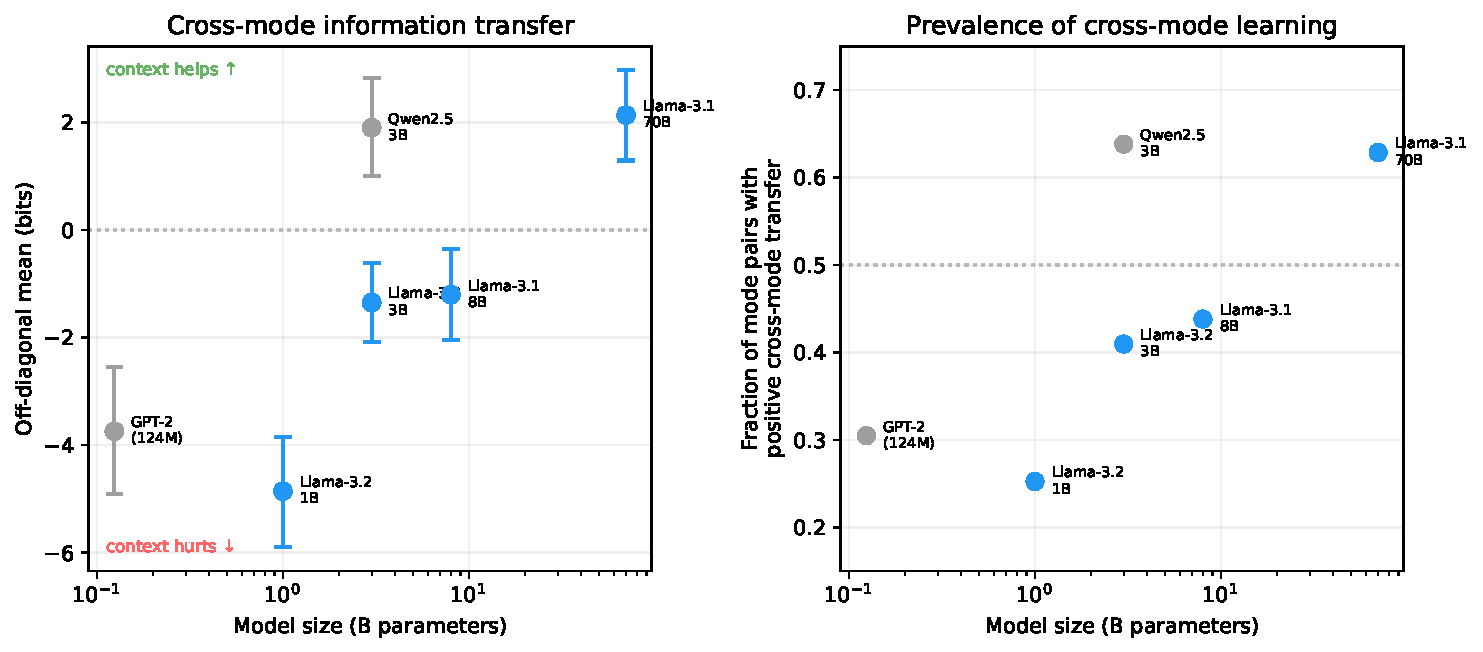
\includegraphics[width=\textwidth]{scaling_comparison/paper_scaling_figure.pdf}
\caption{Cross-mode information transfer scales with model size. \textbf{Left}: Mean off-diagonal surprise reduction (with bootstrap 95\% CI) transitions from negative to positive as models grow, indicating that larger models extract more information from cross-mode context. \textbf{Right}: The fraction of mode pairs showing positive cross-mode transfer increases monotonically across the \scalingNumLlamaModels{} Llama models (blue; $p = \scalingFactorialProbPct\%$ under monotone null).
GPT-2 and Qwen2.5-3B (gray) are included for context but differ in architecture.}
\label{fig:scaling-crossmode}
\end{figure*}

\paragraph{The framework admits other metrics.} The $a_k$ curve is the primary object of our framework, and $D_{Ca_n} = C \times a_n$ is one natural summary of it among many.
Reporting the curve directly preserves information that any single scalar (including ours) collapses.
Alternative scalars could be derived from the same curve to capture different desiderata: weighted sums of $a_k - a_\infty$ (emphasizing early or late positions), the slope or curvature at a specific $k$ (measuring how quickly $\theta$ learns), curve-shape descriptors, or coherence-weighted variants that combine $C$ with quantities other than $a_n$.
Different applications may warrant different choices; for instance, a policy-comparison setting might prefer a metric sensitive to \emph{changes} in the curve shape, while a ranking setting needs a single well-behaved scalar.
We have not explored this space systematically; we focus on $D_{Ca_n}$ because it empirically works well across regimes and has a clean information-theoretic interpretation, but we expect the framework to support a family of related metrics with complementary properties.


\section{Future Work}

Several directions remain unexplored.

\paragraph{Prompt format optimization.} We use a fixed prompt template throughout and do not attempt to optimize it for ICL elicitation.
Prompt engineering could improve the metric's discriminative power.
Dimension-specific framings (e.g., ``Here are several stories in different genres'') are one such variant: priming $\theta$ to expect variation along a dimension removes the small portion of the surprise attributable to the mere existence of that variation, but it does not isolate per-dimension diversity, since the rest of the cross-response surprise reduction remains.

\paragraph{Ensembling base models.} A single base model $\theta$ may produce non-monotone $a_k$ curves when pushed out of distribution by long contexts.
Ensembling multiple base models at the token level (averaging softmax probabilities) could stabilize the estimates while preserving the autoregressive structure.
Our codebase supports token-level ensembling, but we have not yet validated it experimentally.

\paragraph{Total-bits variants of $D$.}
We report $D_{Ca_n} = C \times a_n$ in bits/byte for length control, normalising by bytes rather than tokens so that scores remain tokenizer-agnostic.
The implementation also exposes $a_n$ in total bits, which is likewise tokenizer-agnostic but not length-controlled.
A hybrid scalar $C \times a_n^{\text{bits}}$ rewards length (longer responses have more positions at which to be surprising), which some practitioners may want; characterising when each variant is the appropriate measurement target is left to future work.


\section{Excess Entropy and the \texorpdfstring{$C \times E$}{C x E} Score}\label{app:excess-entropy}

This appendix develops the excess entropy $E$, an alternative summary of the $a_k$ curve that is theoretically interesting (connecting to the excess entropy of computational mechanics \citep{crutchfield2003regularities} and to the total correlation) but empirically inferior to $D_{Ca_n}$ on the external benchmarks of Section~\ref{sec:tevet}.
We include it here for theoretical completeness and to explain the empirical comparisons that motivate our preference for $D_{Ca_n}$.

\subsection{The Excess Entropy}\label{app:excess-entropy-def}

Neither the running average $\bar{a}_n = \frac{1}{n}\sum_k a_k$ nor the total correlation $\TC_n$ is a satisfactory single scalar.
The running average converges to $a_\infty$ (the uninteresting residual floor), losing sensitivity to the learnable structure above it.
The total correlation grows linearly in $n$ and never saturates, because each new term contributes approximately $-\log_2 \theta(r \mid p) - a_\infty > 0$ for large $k$.

The solution is to isolate the signal above the noise floor.
Following the concept of excess entropy from computational mechanics \citep{crutchfield2003regularities}, define the \textbf{excess entropy}:\footnote{The excess entropy $E = \sum_k (a_k - a_\infty)$ is defined as a discrete sum over integer response indices, since ``conditioning on 3.5 responses'' has no direct meaning.
However, a continuous extension exists: consider conditioning on a random subset of size $\alpha n$ for $\alpha \in [0,1]$, yielding a continuous curve $\bar{a}(\alpha)$.
The discrete $\bar{a}_k$ would be samples at $\alpha = k/n$, and $E$ would correspond to integrating this curve (in which case trapezoidal integration would be more faithful than Riemann sums).
We treat $E$ as the discrete sum throughout, but note that the continuous interpretation remains an open question, particularly in connection to the continuous excess entropy literature.
The practical difference between Riemann and trapezoidal sums over $\sim$15 points is small.}
\begin{equation}\label{eq:excess}
    E = \sum_{k=1}^{\infty}\bigl(a_k - a_\infty\bigr)
\end{equation}

Units: bits.
This is the total learnable structural information in the progressive conditioning process, above the irreducible residual noise.
It converges whenever $\theta$'s surprise at new responses eventually stabilizes (since $a_k \to a_\infty$ and the excess $e_k = a_k - a_\infty$ decays to zero).
The ``structure'' captured by $E$ is not limited to discrete mode identity: it includes any inter-response regularity that $\theta$ can learn from context, such as shared stylistic patterns, vocabulary, topic constraints, and formatting conventions.

In practice, $a_\infty$ is unknown.
We estimate it as $a_n$ (the last observed value) and compute:
\begin{equation}\label{eq:excess-hat}
    \hat{E}_n = \sum_{k=1}^{n}(a_k - a_n)
\end{equation}

This underestimates $E$ (since $a_n \geq a_\infty$), but the bias decreases with $n$.

\paragraph{Parametric extrapolation of $a_\infty$.} Rather than using $a_n$ directly, one can fit a parametric model to the observed curve and extrapolate $a_\infty$.
The $a_k$ curve is theoretically expected to be sigmoidal (with concave-up/exponential decay as the degenerate case when the inflection point $k_0 < 1$).
This motivates fitting a four-parameter sigmoid:
\begin{equation}\label{eq:sigmoid-fit}
    a_k = a_\infty + \frac{\alpha}{1 + e^{\beta(k - k_0)}}
\end{equation}
where $a_\infty$ is the asymptotic floor, $\alpha$ is the total drop from $a_1$ to $a_\infty$, $\beta > 0$ controls the steepness of the transition, and $k_0$ is the inflection point.
The fit yields $a_\infty$ without requiring $n$ to be large enough for convergence, and the inflection point $k_0$ provides a principled mode-count estimate when $k_0 > 1$ (Appendix~\ref{app:k0-derivation}).
Section~\ref{sec:mode-count-scaling} provides empirical evidence that the sigmoid-extrapolated $E_{\mathrm{fit}}$ recovers the expected monotonic relationship between mode count and excess entropy, while the raw $\hat{E}_n$ estimator does not.

\paragraph{Relationship to total correlation.} The excess entropy and total correlation are complementary decompositions of the same underlying structure.
Working in expectation over i.i.d.\ draws from $\pi$, let $\bar{a}_1 = \E[-\log_2 \theta(r \mid p)]$ denote the expected unconditional cross-entropy, $\bar{a}_k = \E[a_k]$ the expected conditional cross-entropy at position $k$, and $e_k = \bar{a}_k - a_\infty$ the excess at step $k$.
The per-step mutual information is $I_k = \bar{a}_1 - \bar{a}_k = (\bar{a}_1 - a_\infty) - e_k$.
Summing:
\begin{equation}\label{eq:tc-decomp}
    \TC_n = \sum_{k=1}^{n} I_k = n(\bar{a}_1 - a_\infty) - E_n
\end{equation}

For large $n$ where $E_n \to E$, the total correlation grows linearly with slope $(\bar{a}_1 - a_\infty)$: $\TC_n \approx n(\bar{a}_1 - a_\infty) - E$.
Figure~\ref{fig:decomposition} illustrates.
The three quantities have clean interpretations, all in bits: $(\bar{a}_1 - a_\infty)$ is the per-response redundancy once $\theta$ has fully learned the available structure; $E$ is the total finite structural information, consumed during $\theta$'s transient learning phase; $\TC_n$ is the cumulative redundancy, which grows without bound.

\begin{figure}[tb]
\centering
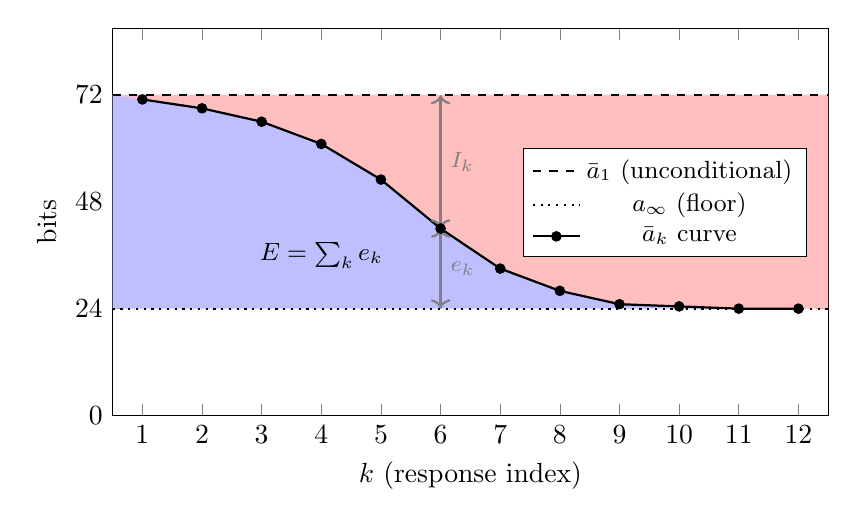
\begin{tikzpicture}
\begin{axis}[
    width=0.88\textwidth,
    height=6.5cm,
    xlabel={$k$ (response index)},
    ylabel={bits},
    xmin=0.5, xmax=12.5,
    ymin=0, ymax=87,
    xtick={1,2,3,4,5,6,7,8,9,10,11,12},
    ytick={0, 24, 48, 72},
    legend style={font=\small, at={(0.97,0.55)}, anchor=east},
    clip=false,
]

% Define h-bar line
\addplot[name path=hbar, forget plot, draw=none]
    coordinates {(0.5,72) (12.5,72)};

% Define a_infinity line
\addplot[name path=ainf, forget plot, draw=none]
    coordinates {(0.5,24) (12.5,24)};

% Define a_k curve (theoretical, in expectation)
\addplot[name path=ak, forget plot, draw=none]
    coordinates {
        (0.5,72) (1,71) (2,69) (3,66) (4,61)
        (5,53) (6,42) (7,33) (8,28) (9,25)
        (10,24.5) (11,24) (12,24) (12.5,24)
    };

% Fill TC area (between h-bar and a_k) — red
\addplot[red!25, forget plot] fill between[of=hbar and ak];

% Fill E area (between a_k and a_infinity) — blue
\addplot[blue!25, forget plot] fill between[of=ak and ainf];

% Draw the visible lines on top
\addplot[thick, dashed, black]
    coordinates {(0.5,72) (12.5,72)};
\addlegendentry{$\bar{a}_1$ (unconditional)}

\addplot[thick, dotted, black]
    coordinates {(0.5,24) (12.5,24)};
\addlegendentry{$a_\infty$ (floor)}

\addplot[thick, black, mark=*, mark size=1.5pt]
    coordinates {
        (1,71) (2,69) (3,66) (4,61)
        (5,53) (6,42) (7,33) (8,28) (9,25)
        (10,24.5) (11,24) (12,24)
    };
\addlegendentry{$\bar{a}_k$ curve}

% Labels for the colored regions
\node[font=\small] at (axis cs:10,55) {$\TC_n = \sum_k I_k$};
\node[font=\small] at (axis cs:4,36) {$E = \sum_k e_k$};

% Annotation arrows showing I_k and e_k for a single step (k=6, a_6=42)
\draw[<->, thick, gray] (axis cs:6,42) -- node[right, font=\footnotesize] {$e_k$} (axis cs:6,24);
\draw[<->, thick, gray] (axis cs:6,72) -- node[right, font=\footnotesize] {$I_k$} (axis cs:6,42);

\end{axis}
\end{tikzpicture}
\caption{Decomposition of the gap between unconditional surprise $\bar{a}_1$ and the asymptotic floor $a_\infty$ at each step $k$.
The per-step gap $\bar{a}_1 - a_\infty$ splits into mutual information $I_k = \bar{a}_1 - \bar{a}_k$ (\textcolor{red!70}{red}, above the curve) and excess $e_k = \bar{a}_k - a_\infty$ (\textcolor{blue!70}{blue}, below the curve).
Summing across $k$: the red area is the total correlation $\TC_n$; the blue area is the excess entropy $E$.
As $k$ grows, $e_k \to 0$ and each step contributes the full $\bar{a}_1 - a_\infty$ to $\TC_n$, so $\TC_n$ grows linearly while $E$ converges.
All quantities are in bits.}
\label{fig:decomposition}
\end{figure}

\subsection{Per-Byte Excess Entropy Rate}\label{app:per-byte-rate}

The excess entropy $E = \sum_k (a_k - a_\infty)$ is in bits.
For a length-normalized variant, we define the \textbf{per-byte excess entropy rate} by normalizing each response's surprise by its byte count \emph{before} averaging across permutations.
For a single permutation $\sigma$, the per-byte conditional surprise at position $k$ is $a_k^\sigma / \|r_{\sigma(k)}\|$ (bits/byte).
Averaging over permutations gives
\begin{equation}
    \hat{a}_k^{\mathrm{rate}} = \E_\sigma\!\left[\frac{a_k^\sigma}{\|r_{\sigma(k)}\|}\right]
\end{equation}
and the per-byte floor is estimated analogously from the last position: $\hat{a}_\infty^{\mathrm{rate}} = \hat{a}_n^{\mathrm{rate}}$.
The per-byte excess entropy rate is
\begin{equation}\label{eq:per-byte-E}
    E_{\mathrm{rate}} = \sum_{k=1}^{n}\bigl(\hat{a}_k^{\mathrm{rate}} - \hat{a}_\infty^{\mathrm{rate}}\bigr).
\end{equation}
This treats each response equally regardless of length.
Note that $E_{\mathrm{rate}} \neq E / \bar{B}$ in general: because total surprise $a_k$ and byte count $\|r_k\|$ are positively correlated, $E / \bar{B}$ overweights long responses, while the per-response normalization in $E_{\mathrm{rate}}$ avoids this.

\subsection{The \texorpdfstring{$C \times E$}{C x E} Score}

Combining $E$ with the coherence term $C$ (Section~\ref{sec:coherence}) yields scalar scores
\begin{equation}\label{eq:D-total}
    C \times E \quad \text{(bits)} \qquad \text{or} \qquad C \times E_{\mathrm{rate}} \quad \text{(bits/byte)}.
\end{equation}
The first weights total structural information by per-byte plausibility; the second normalizes per byte so long and short responses are treated equally.

\subsection{Why Not Weight Excess Entropy Inside the Sum?}\label{app:why-not-weight}

A natural alternative to reporting $E$ and $C$ separately is to weight the terms within $E$ by coherence, computing $E_w = \sum_k w_k \cdot (a_k - a_\infty)$ where $w_k = 2^{-h_\theta(r_k \mid p)}$.
This would suppress contributions from incoherent modes directly at the point of measurement.
We considered and rejected this approach for three reasons.
First, it breaks the information-theoretic interpretation: $E = \sum_k e_k$ has a clean meaning as the total structural information above the noise floor, connected to Crutchfield and Feldman's excess entropy, and inserting weights makes $E_w$ a hybrid quantity that is not the excess entropy of any well-defined process.
Second, the weights are not independent of what they weight: both $w_k$ and $e_k$ are derived from the same response scored by the same model, and an incoherent response from a novel mode has both high $e_k$ and low $w_k$, which partially cancel in ways that lack a clean characterization.
Third, it makes the noise floor $a_\infty$ ambiguous: unclear whether it should also be weighted, and if so by what.

\subsection{Limitations of $C \times E$}

$C \times E$ inherits two limitations from $E$.
First, $E$ measures learnable \emph{structure} (recurring patterns that $\theta$ can extract from seeing multiple responses) rather than continuous spread.
A policy that draws from a broad, roughly continuous distribution of coherent outputs has $a_k \approx a_1$ for all $k$, yielding $E \approx 0$ despite maximal diversity.
Second, $E$ is near-zero in the few-draws regime: with only 5--10 responses and no repeated modes, $\theta$ finds little learnable structure regardless of diversity, so $C \times E$ carries almost no signal.
These limitations are the reason $D_{Ca_n}$ is preferred as the primary score: $a_\infty$ is the \emph{level} of the floor, which differs meaningfully between diverse and non-diverse response sets even when the curve stays nearly flat.

\paragraph{Empirical inferiority.} On Tevet's diversity-eval benchmark with only 5 responses per set (Section~\ref{sec:tevet}), $C \times a_n$ achieves ROC AUC of \tevetMcDivNugPromptGenCxAnAUC{} on McDiv\_nuggets prompt\_gen while the $D_{\mathrm{fit}} = C \times E_{\mathrm{fit}}$ variant cannot be computed at all (the four-parameter sigmoid fails to converge on only five points) and the discretized $D_{\mathrm{disc}}$ variant is anti-correlated with diversity (AUC = \tevetMcDivNugPromptGenDdiscAUC{}, well below chance).
Figure~\ref{fig:roc-curves} shows the ROC curves.

\begin{figure}[h]
\centering

\includegraphics[width=\textwidth]{tevet_validation/c_ainf_analysis_v3/roc_curves_mcdiv_nuggets.png}
\caption{ROC curves for McDiv\_nuggets binary classification (Qwen2.5-3B, 50 permutations).
Five per-byte metrics are overlaid per panel: $C \times a_n$ (red, solid), $a_n$ alone (orange, dashed), $D_{\mathrm{fit}} = C \times E_{\mathrm{fit}}$ (blue, solid), $D_{\mathrm{disc}} = C \times \hat{E}_n$ (cyan, dashed), and $a_1$ (gray, dotted). Line style is redundant with color so the encoding remains legible under common color-vision deficiencies.
$C \times a_n$ dominates the other four scores on every task; the $E$-based scores ($D_{\mathrm{fit}}, D_{\mathrm{disc}}$) hug or fall below the chance diagonal in this 5-response regime.}
\label{fig:roc-curves}
\end{figure}

\paragraph{Why $E$ fails in this regime.} With only 5 responses and no repeated modes, $\theta$ finds little learnable structure regardless of diversity.
The $a_k$ curve stays approximately flat, yielding $E \approx 0$ for both diverse and non-diverse sets.
The $E$-based scores thus carry almost no signal.
The asymptotic floor $a_\infty$, by contrast, differs substantially between the two conditions: diverse responses remain surprising after conditioning ($a_\infty$ high), while paraphrases become predictable ($a_\infty$ low).
This is the fundamental reason $D_{Ca_n}$ is preferred.

\subsection{Coherence Normalization Strategies}\label{app:c-normalization}

Two strategies are available when coherence variation dominates diversity variation:
\begin{enumerate}[nosep]
    \item \textbf{Normalization}: Replace $C$ with $C / C_{\mathrm{base}}$, where $C_{\mathrm{base}}$ is the coherence of $\theta$'s own samples given the same prompt.
The ratio lives in $(0, 1]$ and equals 1 when $\pi$ is as coherent as $\theta$, removing the baseline suppression.
This has a clean interpretation as ``what fraction of baseline coherence does $\pi$ retain?''
    \item \textbf{Fractional exponent}: Replace $C$ with $C^\alpha$ for $\alpha \in (0, 1)$, which compresses the coherence penalty.
This softens the dominance of $C$ but introduces a free hyperparameter without information-theoretic motivation.
\end{enumerate}
We recommend normalization when a single-scalar ranking is the primary use case, and the unmodified $C$ when the goal is diagnostic.
We did not use either strategy in our experiments.

\subsection{Mode Count Scaling: Excess-Entropy Metrics}

In the synthetic mode count experiments (Section~\ref{sec:mode-count-scaling}), the sigmoid-extrapolated $E_{\mathrm{fit}}$ is monotonic in mode count for Qwen2.5-3B but has wide confidence intervals at high $m$, while the raw $\hat{E}_n$ estimator is non-monotonic.
Table~\ref{tab:mode-count} and Figure~\ref{fig:metrics-vs-m} show the details.

\begin{table}[h]
\centering
\caption{Mode count scaling metrics for Qwen2.5-3B ($n=\modeCountNResponses$, \modeCountNDraws{} draws). $E_{\mathrm{fit}}$ is the sigmoid-extrapolated excess entropy; $a_n$ is the mean floor at $k=\modeCountNResponses$; $\sigma_\ell$ is per-byte coherence spread; $k_0$ is the sigmoid inflection point.
Confidence intervals are 95\% bootstrap.}
\label{tab:mode-count}
\small
% Generated by: scripts/generate_mode_count_table.py
% Data source: results/mode_count/qwen2.5-3b_1k_draws.json
%              results/mode_count/qwen2.5-3b_fits.json
\begin{tabular}{@{}r rrrr@{}}
\toprule
$m$ & $E_{\mathrm{fit}}$ (bits) & $a_n$ (bits) & $\sigma_\ell$ (bits/byte) & $k_0$ \\
\midrule
1  & $296 \pm 11$ & 9.3 & 0.1 & $-10.0$ \\
2  & $568 \pm 24$ & 16.9 & 0.2 & $-10.0$ \\
3  & $704 \pm 40$ & 26.7 & 0.2 & $-10.0$ \\
4  & $799 \pm 67$ & 37.4 & 0.3 & $-10.0$ \\
5  & $855 \pm 113$ & 48.0 & 0.3 & $-10.0$ \\
6  & $940 \pm 127$ & 56.1 & 0.3 & $-10.0$ \\
7  & $1069 \pm 194$ & 61.5 & 0.3 & $-10.0$ \\
8  & $1138 \pm 253$ & 66.9 & 0.3 & $-10.0$ \\
9  & $1563 \pm 705$ & 72.8 & 0.3 & $-10.0$ \\
10  & $1807 \pm 1194$ & 77.8 & 0.3 & $-10.0$ \\
\bottomrule
\end{tabular}

\end{table}

\begin{figure}[h]
\centering

\includegraphics[width=0.6\textwidth]{mode_count/qwen2.5-3b/metrics_vs_m.png}
\caption{Summary metrics vs.\ mode count $m$ (Qwen2.5-3B, $n=\modeCountNResponses$, \modeCountNDraws{} draws). $E_{\mathrm{fit}}$ (sigmoid-extrapolated) increases monotonically, while the raw $\hat{E}_n$ does not.}
\label{fig:metrics-vs-m}
\end{figure}

\begin{figure}[h]
\centering

\includegraphics[width=0.6\textwidth]{mode_count/qwen2.5-3b/fit_params_vs_m.png}
\caption{Sigmoid fit parameters vs.\ mode count $m$ (Qwen2.5-3B).
The inflection point $k_0$ remains at the lower bound ($-10$) across all $m$, indicating pure exponential decay without an initial plateau (see Section~\ref{sec:cross-mode-learning}).}
\label{fig:fit-params}
\end{figure}

% Generated by scripts/dataset_confound_analysis.py
% Per-byte a_1 for r_0 of the illustrative high- and low-diversity samples.
% high sample: test.sa-sb.sa::00698
% low sample:  test.sa-sb.sa-b::00279
\newcommand{\confoundHighRoAone}{0.783}
\newcommand{\confoundLowRoAone}{1.777}
\newcommand{\confoundHighSampleId}{test.sa-sb.sa::00698}
\newcommand{\confoundLowSampleId}{test.sa-sb.sa-b::00279}


\section{Dataset Construction Confounds in McDiv}\label{app:confound}

When validating against the McDiv\_nuggets benchmark \citep{tevet2020evaluating}, we observed that the mean $\bar{a}_1$ curve (per-byte) for the ``low diversity'' group starts \emph{above} the ``high diversity'' group in the story\_gen task (Figure~\ref{fig:confound-a1-dist}).
Since $a_1$ measures the surprise of the first response conditioned only on the prompt (before any other responses appear in context), this gap cannot reflect diversity.
It is a confound in the dataset construction.

\subsection{Mechanism}

The McDiv\_nuggets protocol (Tevet and Berant \S6.4) pairs a low-diversity set with each high-diversity set as follows.
Workers first write five \emph{different} continuations (the high-diversity set).
The same worker is then asked to \emph{self-select one} of their own five responses and paraphrase it five times, preserving content while varying form (the low-diversity set).
Tevet and Berant do not characterize the distribution of which responses workers self-select.

Empirically (see Table~\ref{tab:confound-stats} and Figure~\ref{fig:confound-a1-dist}, and the illustrative examples from the McDiv\_nuggets story\_gen dataset in Section~\ref{sec:mcdiv-examples} below), we observe that the self-selected endings for the low-diversity sets tend to be more specific or dramatic (e.g., ``He scored winner'' or ``they quit'') than the typical high-diversity continuations (e.g., ``Joel fired the cook when things went too far downhill'').
This means that individual low-diversity responses are intrinsically more surprising to the base model, not because of diversity, but because of the specificity of the endings workers self-selected for paraphrasing.

\subsection{Evidence}

Table~\ref{tab:confound-stats} summarizes the gap.
The per-byte $a_1$ difference is substantial (a content effect) while the total-bits difference is small because high-diversity responses are on average several bytes longer.

\begin{table*}[ht]
\centering
\caption{Unconditional surprise ($a_1$) by diversity label, McDiv\_nuggets story\_gen.}\label{tab:confound-stats}
% Generated by scripts/dataset_confound_analysis.py
% Source: results/tevet/qwen25_completion_v3/McDiv_nuggets/*_with_hds_story_gen.csv
\begin{tabular}{lccc}
\toprule
 & High diversity & Low diversity & Gap \\
\midrule
$a_1$ (bits/byte) & 0.977 & 1.154 & +0.177 \\
$a_1$ (total bits) & 49.1 & 50.5 & +1.4 \\
Mean response bytes & 52.7 & 46.5 & $-6.3$ \\
$n$ & 103 & 97 & \\
\bottomrule
\end{tabular}

\end{table*}

The gap persists after binning by response length (Table~\ref{tab:confound-length}), confirming it is primarily a content effect rather than a length artifact: the high-minus-low per-byte gap remains positive across the bulk of the length range.

\begin{table*}[ht]
\centering
\caption{Unconditional per-byte surprise by response length bin, story\_gen.}\label{tab:confound-length}
% Generated by scripts/dataset_confound_analysis.py
% Source: results/tevet/qwen25_completion_v3/McDiv_nuggets/*_with_hds_story_gen.csv
\begin{tabular}{lccl}
\toprule
Byte range & High div.\ mean & Low div.\ mean & Gap \\
\midrule
$[20, 40)$ & 1.172 & 1.340 & +0.167 \\
$[40, 60)$ & 0.878 & 1.019 & +0.141 \\
$[60, 80)$ & 0.853 & 1.029 & +0.176 \\
$[80, 120)$ & 0.905 & 0.908 & +0.003 \\
\bottomrule
\end{tabular}

\end{table*}

\subsection{Illustrative Examples}\label{sec:mcdiv-examples}

Figures~\ref{fig:confound-high} and~\ref{fig:confound-low} show per-token surprise (in bits) for the first response of a high-diversity and low-diversity sample, respectively.
Samples are drawn by ranking each label group by per-byte $a_1$ (ascending for high-diversity, descending for low-diversity) and taking the sample at the $\lfloor N/4 \rfloor$ position, chosen to be representative of the expected confound direction rather than an extreme outlier; the specific pinned IDs (\texttt{sa\_00698}, \texttt{sa-b\_00279}) are fixed in \texttt{scripts/dataset\_confound\_analysis.py} for reproducibility.
Red bars are measured response tokens; grey bars are masked context tokens.

\paragraph{High diversity} (Figure~\ref{fig:confound-high}).
Context: \emph{``Joel owned a restaurant.
He hired a cook that didn't care about his work.
The cook didn't clean after himself.
The kitchen was a mess.''} Response: \emph{``Joel fired the cook when things went too far downhill.''} This is a natural, predictable continuation ($a_1 = \confoundHighRoAone$ bits/byte).

\paragraph{Low diversity} (Figure~\ref{fig:confound-low}).
Context: \emph{``Harry and his basketball team was losing the game.
The coach called for a timeout.
Harry boosted morale by talking to his team.
The team caught up and the game was tied.''} Response: \emph{``He scored winner.''} This is a specific, somewhat ungrammatical ending ($a_1 = \confoundLowRoAone$ bits/byte).
All five responses in this set are paraphrases of the same idea (``Harry scored the winning point'').

\begin{figure*}[h]
\centering
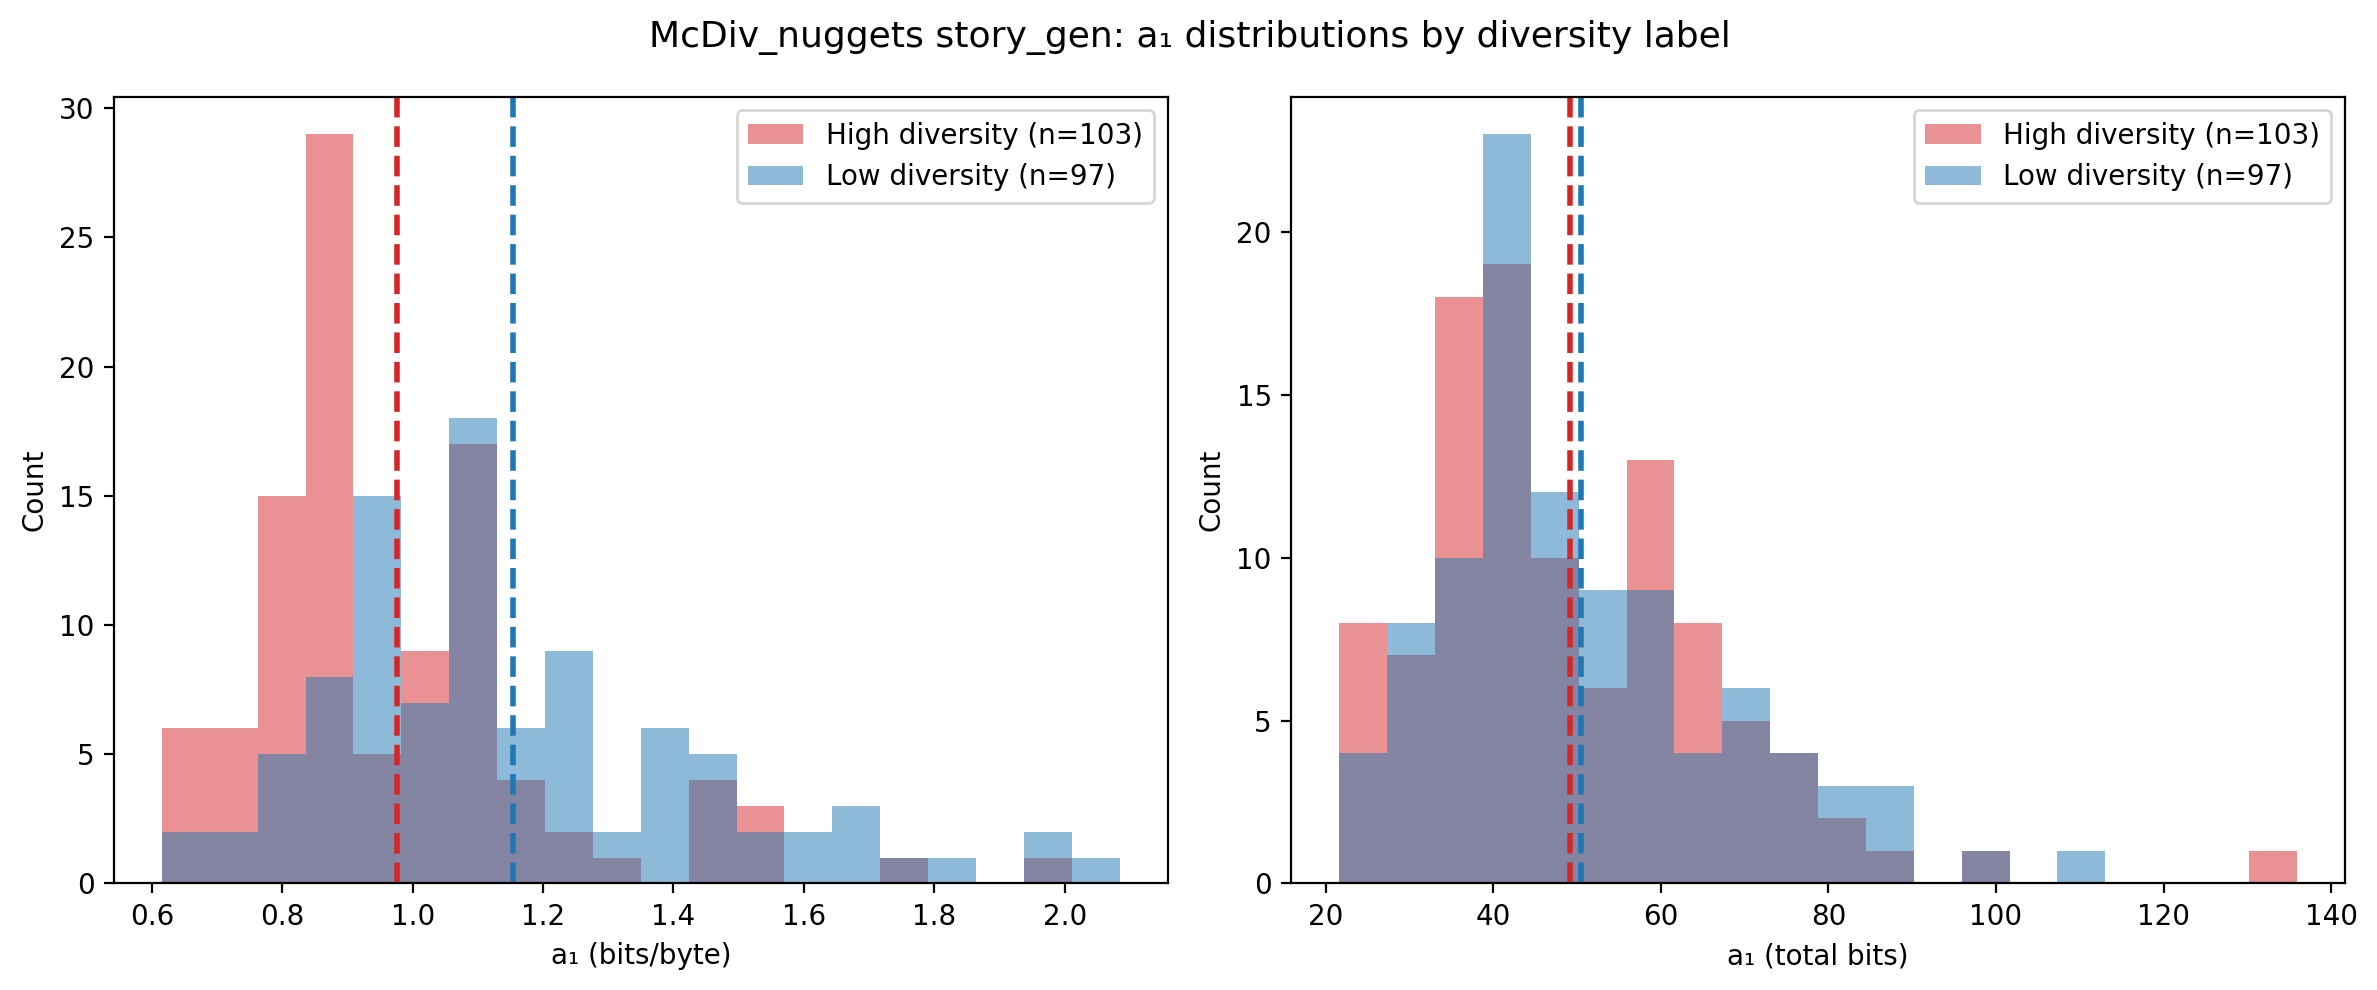
\includegraphics[width=\textwidth]{../figures/dataset_confound/a1_distributions.png}
\caption{Distribution of $a_1$ (unconditional surprise of the first response) for high- vs.\ low-diversity story\_gen samples.
Left: per-byte.
Right: total bits.
The per-byte gap (see Table~\ref{tab:confound-stats}) is a dataset construction artifact.}\label{fig:confound-a1-dist}
\end{figure*}

\begin{figure*}[h]
\centering
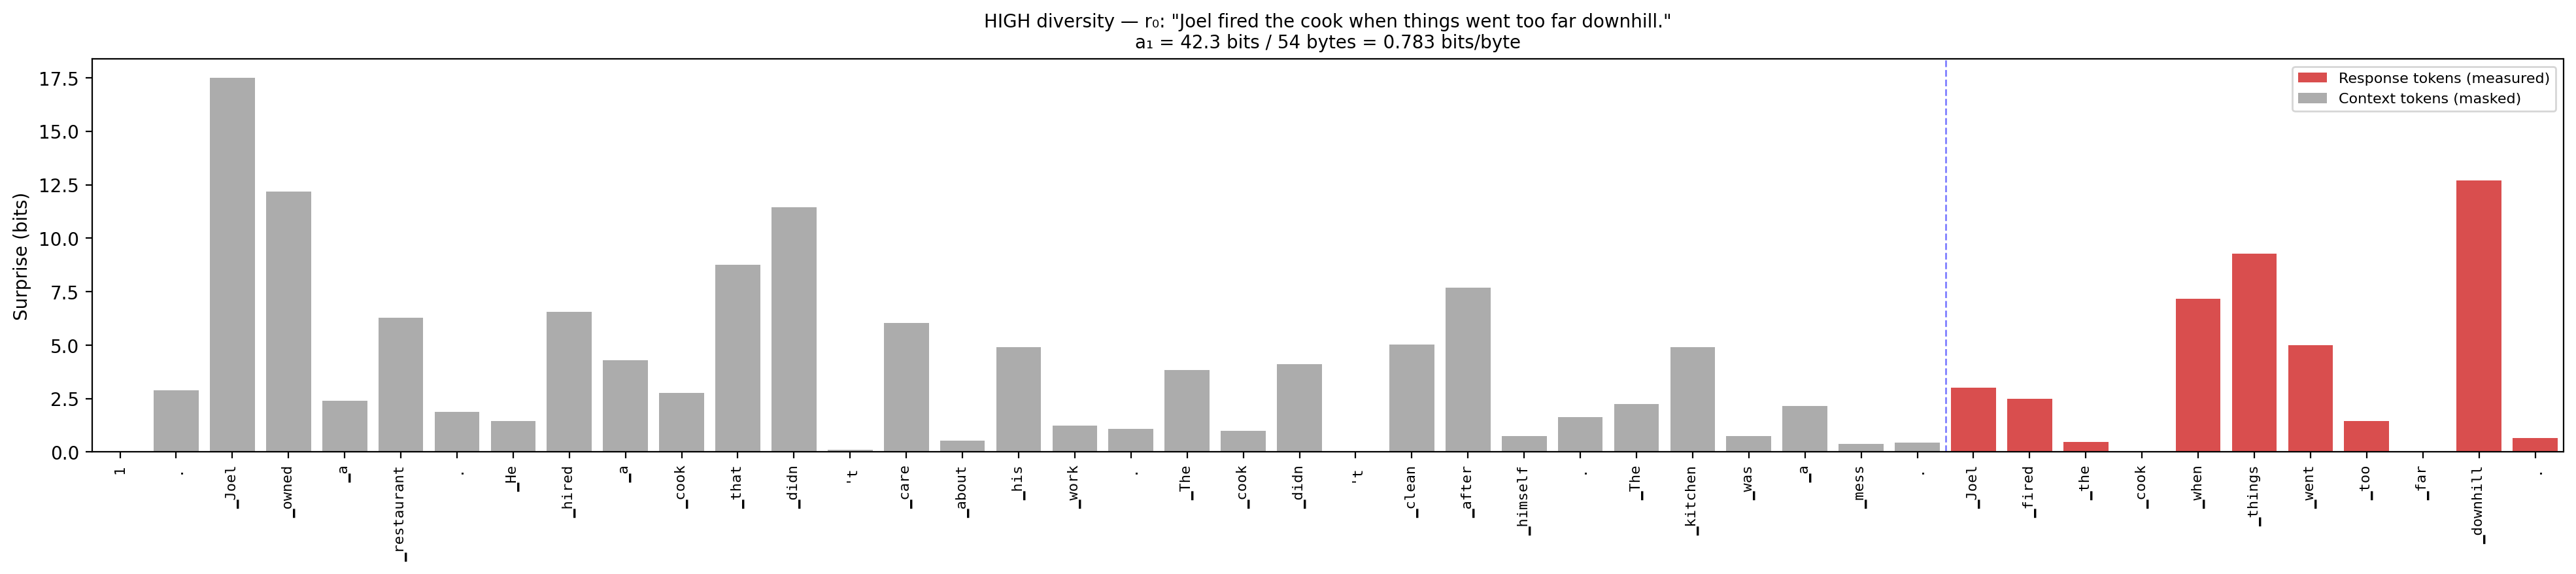
\includegraphics[width=\textwidth]{../figures/dataset_confound/per_token_high_0_test.sa-sb.sa_00698.png}
\caption{Per-token surprise for a high-diversity sample's first response.
The continuation (``Joel fired the cook...'') is predictable, yielding low per-token surprise across response tokens.}\label{fig:confound-high}
\end{figure*}

\begin{figure*}[h]
\centering
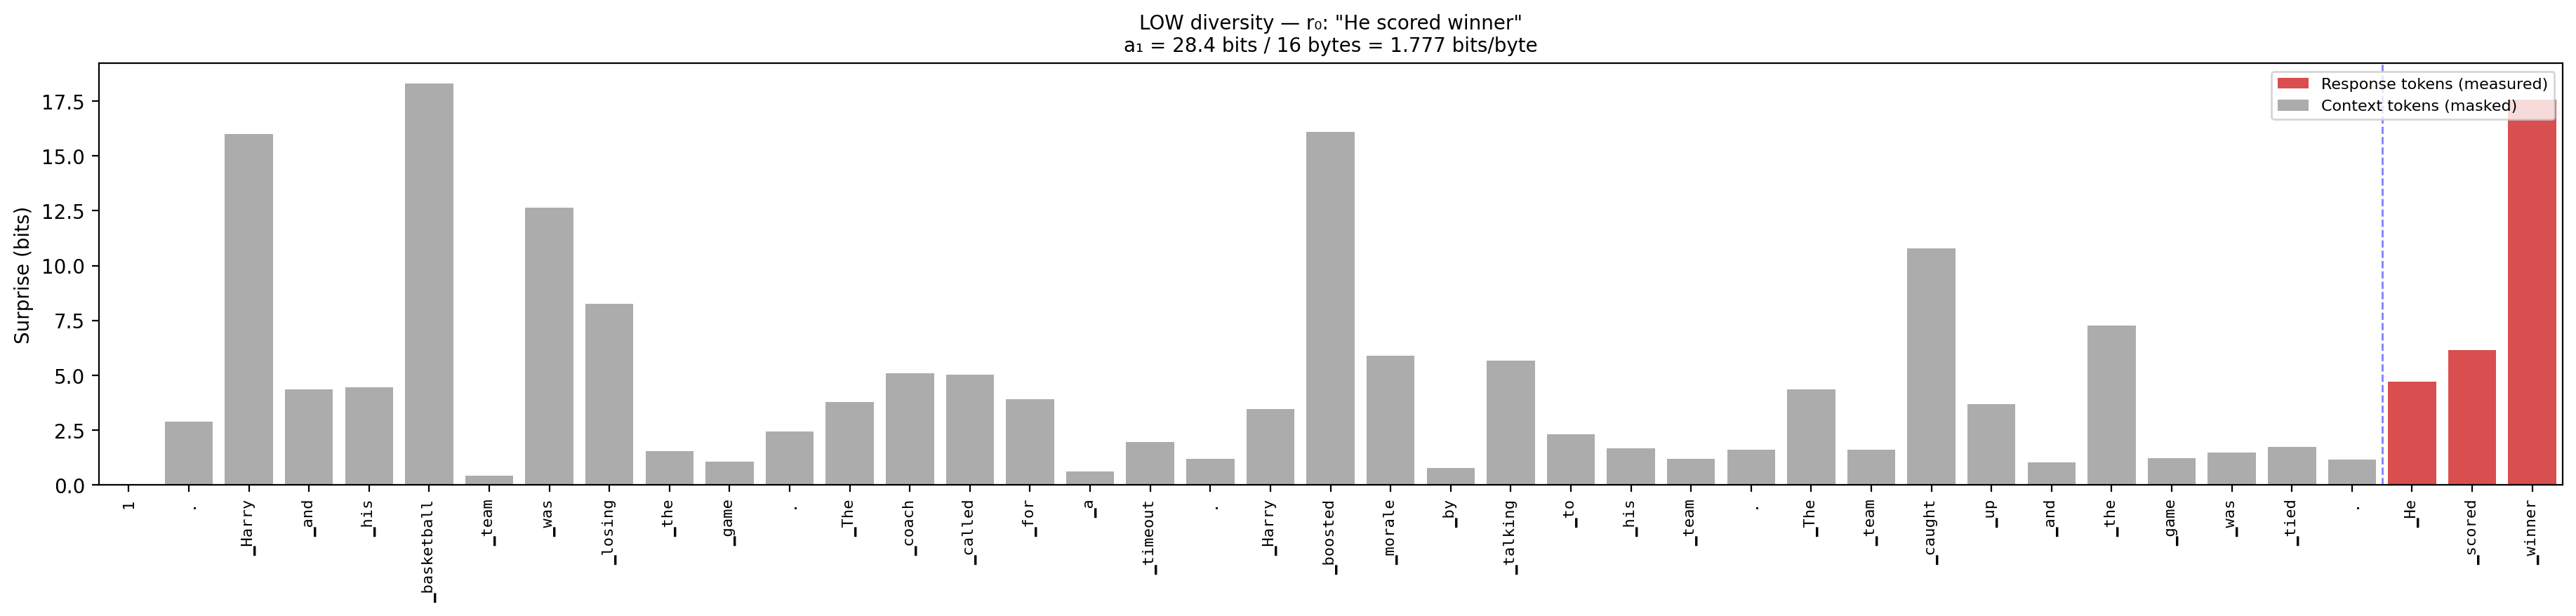
\includegraphics[width=\textwidth]{../figures/dataset_confound/per_token_low_0_test.sa-sb.sa-b_00279.png}
\caption{Per-token surprise for a low-diversity sample's first response.
The specific ending (``He scored winner'') is inherently more surprising to the base model, despite being labeled ``low diversity.''}\label{fig:confound-low}
\end{figure*}

\subsection{Label Contamination}

In addition to the construction confound, we found that the McDiv\_nuggets CSVs contain duplicate sample IDs with \emph{conflicting labels}: the same response set appears once labeled as high diversity and once as low diversity.
Table~\ref{tab:contamination} shows the extent of this contamination across the three generation tasks.

\begin{table*}[ht]
\centering
\caption{Number of sample IDs appearing with both high- and low-diversity labels in the McDiv\_nuggets (with HDS) CSVs.}\label{tab:contamination}
% Generated by scripts/dataset_confound_analysis.py
% Source: results/tevet/qwen25_completion_v3/McDiv_nuggets/*_with_hds_*.csv
\begin{tabular}{lcc}
\toprule
Task & Conflicting IDs & Total rows \\
\midrule
prompt\_gen & 9 & 200 \\
resp\_gen & 11 & 200 \\
story\_gen & 7 & 200 \\
\bottomrule
\end{tabular}

\end{table*}

These duplicates introduce noise into any correlation analysis: the same $\bar{a}_k$ curve is counted as evidence for \emph{both} labels, diluting the signal.
We did not remove these duplicates from our analysis, so the correlations reported here are conservative.

\subsection{Implications}

This confound does not invalidate McDiv\_nuggets for evaluating diversity metrics, but it does introduce a systematic bias: any metric based on per-response surprise will tend to assign higher values to the low-diversity group, counteracting the expected positive correlation between the metric and the diversity label.
Metrics that compare \emph{across} responses within a set (like excess entropy $E$) are less affected because the confound is approximately constant across positions $k$: it shifts the entire $\bar{a}_k$ curve vertically without changing its shape.
Per-byte normalization amplifies the confound because shorter low-diversity responses get higher bits-per-byte values.


\section{Aggregation Across Prompts}\label{app:aggregation}

This appendix concerns aggregation across prompts.
Aggregation \emph{within} a single prompt, across permutations of the response ordering, is described in Section~\ref{sec:ordering} and given by Eq.~\eqref{eq:akbar-mor}: the per-byte $\bar{a}_k$ is a mean of per-permutation per-byte rates, not a ratio of permutation-averaged bits to permutation-averaged byte counts.\footnote{An earlier revision of our implementation computed the ratio-of-means form, in which the bits and byte counts at each position are each averaged across permutations before dividing.
After enough permutations, the byte counts at each position approach the mean response length, so that estimator collapses into the total-bits curve rescaled by a single constant, losing the per-permutation per-byte signal that Eq.~\eqref{eq:akbar-mor} preserves.
Switching the implementation to the form in Eq.~\eqref{eq:akbar-mor} shifts the headline numbers in this paper by 0--17\% (in mean-of-ratios' favor), with no qualitative change to any ranking we report.}

The diversity score $D_{Ca_n}$ is defined relative to a single prompt $p$.
To summarize a policy's diversity across a prompt suite $P = \{p_1, \ldots, p_M\}$, one can average:
\begin{equation}
    \bar{D}_{Ca_n}(\pi) = \frac{1}{M}\sum_{j=1}^{M} D_{Ca_n}(\pi, p_j)
\end{equation}

To compare two policies $\pi_1$ and $\pi_2$, the natural scalar is the difference:
\begin{equation}
    \Delta D_{Ca_n} = \bar{D}_{Ca_n}(\pi_1) - \bar{D}_{Ca_n}(\pi_2)
\end{equation}

$\Delta D_{Ca_n}$ answers ``how much more plausibility-weighted residual diversity does $\pi_1$ have than $\pi_2$, on average across prompts?''
No division is involved, so $\Delta D_{Ca_n}$ is stable even when either policy's score is near zero.
\section{Scaling the Base Model: Qwen2.5-3B vs Qwen3-30B-A3B-Base}\label{app:qwen3-comparison}

To test whether a stronger base model improves the metric on Tevet's benchmarks, we re-ran the full evaluation using Qwen3-30B-A3B-Base (a 30B-parameter mixture-of-experts model with $\sim$3B active parameters per token) via the Tinker API, with the same setup as in Section~\ref{sec:tevet}: completion-format prompting, 50 permutations, no fine-tuning.
Table~\ref{tab:qwen3-comparison} reports per-task $C \times a_n$ (per-byte) for both base models.

\begin{table}[h]
\centering
\caption{Per-task comparison of $C \times a_n$ (per-byte) for Qwen2.5-3B vs Qwen3-30B-A3B-Base on Tevet diversity-eval. $\Delta$AUC is positive when the larger model wins.
ROC AUC is reported for the binary tasks (McDiv, McDiv\_nuggets, ConTest); only Spearman $\rho$ is meaningful for DecTest (continuous temperature labels).}
\label{tab:qwen3-comparison}
\small
% Generated by: scripts/compare_qwen_models.py --emit-latex
% Data sources: figures/tevet_validation/c_ainf_analysis_v3/summary_table.txt
%               figures/tevet_validation/c_ainf_analysis_qwen3/summary_table.txt
% Metric: C x a_n (per-byte). Q2.5-3B = Qwen2.5-3B local; Q3-30B = Qwen3-30B-A3B-Base via Tinker.
\begin{tabular}{@{}llrrrrr@{}}
\toprule
 &  & \multicolumn{2}{c}{Qwen2.5-3B} & \multicolumn{2}{c}{Qwen3-30B-A3B} & \\
\cmidrule(lr){3-4} \cmidrule(lr){5-6}
Section & Task & $\rho$ & AUC & $\rho$ & AUC & $\Delta$AUC \\
\midrule
McDiv & prompt\_gen (no\_hds) & 0.729 & 0.921 & 0.718 & 0.915 & -0.006 \\
 & resp\_gen (no\_hds) & 0.500 & 0.788 & 0.483 & 0.779 & -0.009 \\
 & story\_gen (no\_hds) & 0.523 & 0.802 & 0.493 & 0.785 & -0.017 \\
\midrule
McDiv\_nuggets & prompt\_gen (no\_hds) & 0.636 & 0.867 & 0.615 & 0.855 & -0.012 \\
 & prompt\_gen (with\_hds) & 0.683 & 0.895 & 0.655 & 0.878 & -0.017 \\
 & resp\_gen (no\_hds) & 0.345 & 0.699 & 0.325 & 0.687 & -0.012 \\
 & resp\_gen (with\_hds) & 0.437 & 0.753 & 0.425 & 0.746 & -0.007 \\
 & story\_gen (no\_hds) & 0.317 & 0.683 & 0.293 & 0.669 & -0.014 \\
 & story\_gen (with\_hds) & 0.405 & 0.734 & 0.376 & 0.717 & -0.017 \\
\midrule
ConTest & prompt\_gen (with\_hds) & 0.584 & 0.837 & 0.592 & 0.842 & +0.005 \\
 & resp\_gen (with\_hds) & 0.391 & 0.726 & 0.333 & 0.692 & -0.034 \\
 & story\_gen (with\_hds) & 0.686 & 0.896 & 0.653 & 0.877 & -0.019 \\
\midrule
DecTest & prompt\_gen (no\_hds) & 0.842 & --- & 0.877 & --- & --- \\
 & prompt\_gen (with\_hds) & 0.845 & --- & 0.875 & --- & --- \\
 & resp\_gen (no\_hds) & 0.771 & --- & 0.804 & --- & --- \\
 & resp\_gen (with\_hds) & 0.760 & --- & 0.777 & --- & --- \\
 & story\_gen (no\_hds) & 0.763 & --- & 0.771 & --- & --- \\
 & story\_gen (with\_hds) & 0.785 & --- & 0.785 & --- & --- \\
\bottomrule
\end{tabular}

\end{table}

\paragraph{Result: scaling did not help on the binary tasks.} On the \qwenThreeBinaryTotal{} binary classification tasks (McDiv, McDiv\_nuggets, ConTest), Qwen2.5-3B wins on \qwenThreeBinaryWinsQwenTwoFive{} of \qwenThreeBinaryTotal{}, with ConTest prompt\_gen the only marginal win for Qwen3-30B-A3B ($\qwenThreeConTestPromptGenDeltaAUC$ AUC).
The mean degradation from scaling is small but consistent (mean $\Delta$AUC = $\qwenThreeBinaryMeanDeltaAUC$ across the \qwenThreeBinaryTotal{} binary tasks).
On the \qwenThreeDecTestTotal{} DecTest tasks (continuous temperature labels), Qwen3-30B-A3B is mildly better on \qwenThreeDecTestWins{} of \qwenThreeDecTestTotal{} (mean $\qwenThreeDecTestMeanDeltaRho$ in Spearman $\rho$, with one tie).

\paragraph{Interpretation.} A natural reading is that the binary McDiv/ConTest labels have low information content: they distinguish only ``high'' vs ``low'' diversity, and this distinction is coarse enough that a 3B base model already captures the relevant signal.
A larger model has nothing more to extract that the binary label can reward.
The continuous DecTest labels are noise-free (temperature is the ground truth), so additional metric resolution from a larger model translates into measurable correlation gains.
If this interpretation is correct, the binary tasks are saturated for our metric and the path to improvement runs through finer-grained labels rather than larger base models.

\paragraph{Caveat: prompt structure was not optimized.} We made no attempt to optimize the prompt structure used to elicit ICL on these benchmarks; the formatting follows the neutral template from Section~\ref{sec:practical} verbatim.
A targeted prompt structure (e.g., explicitly framing the responses as ``Five high-diversity continuations,'' or providing in-context exemplars of diverse vs.\ repetitive sets) would likely improve the metric's discriminative power, particularly for the larger model whose ICL capabilities benefit more from carefully constructed contexts.
We leave prompt-structure optimization to future work.


\section{Cross-Metric Agreement on the OLMo-2-7B RLHF Experiment}\label{app:rlhf-cross-metric}

The RLHF case study (Section~\ref{sec:rlhf-experiment}) reports the headline monotone $D_{Ca_n}$ drop in Table~\ref{tab:rlhf-diversity} and Figure~\ref{fig:rlhf-ak-violin}.
Figure~\ref{fig:rlhf-metric-scatter} plots $D_{Ca_n}$ against the lexical (EAD) and semantic (SentBERT) baselines on the same length-matched subset, confirming that the three metrics see the same diversity-loss signal.

\IfFileExists{../figures/rlhf_experiment/metric_correlation_scatter_alpacaeval_lm.pdf}{%
\begin{figure*}[!htbp]
\centering
\begin{subfigure}[t]{\textwidth}
    \centering
    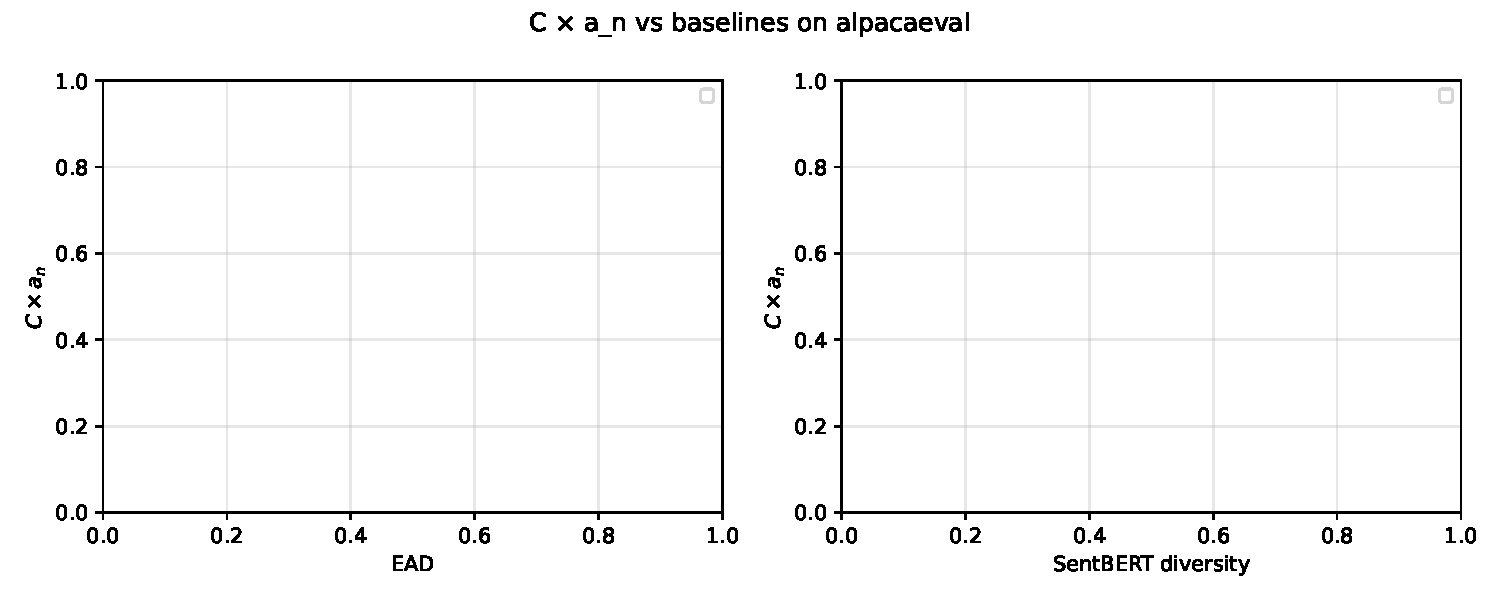
\includegraphics[width=0.85\textwidth]{../figures/rlhf_experiment/metric_correlation_scatter_alpacaeval_lm.pdf}
    \caption{AlpacaEval (length-matched, $n=\olmoLmAlpacaN$ prompts).}
\end{subfigure}\\[0.5em]
\begin{subfigure}[t]{\textwidth}
    \centering
    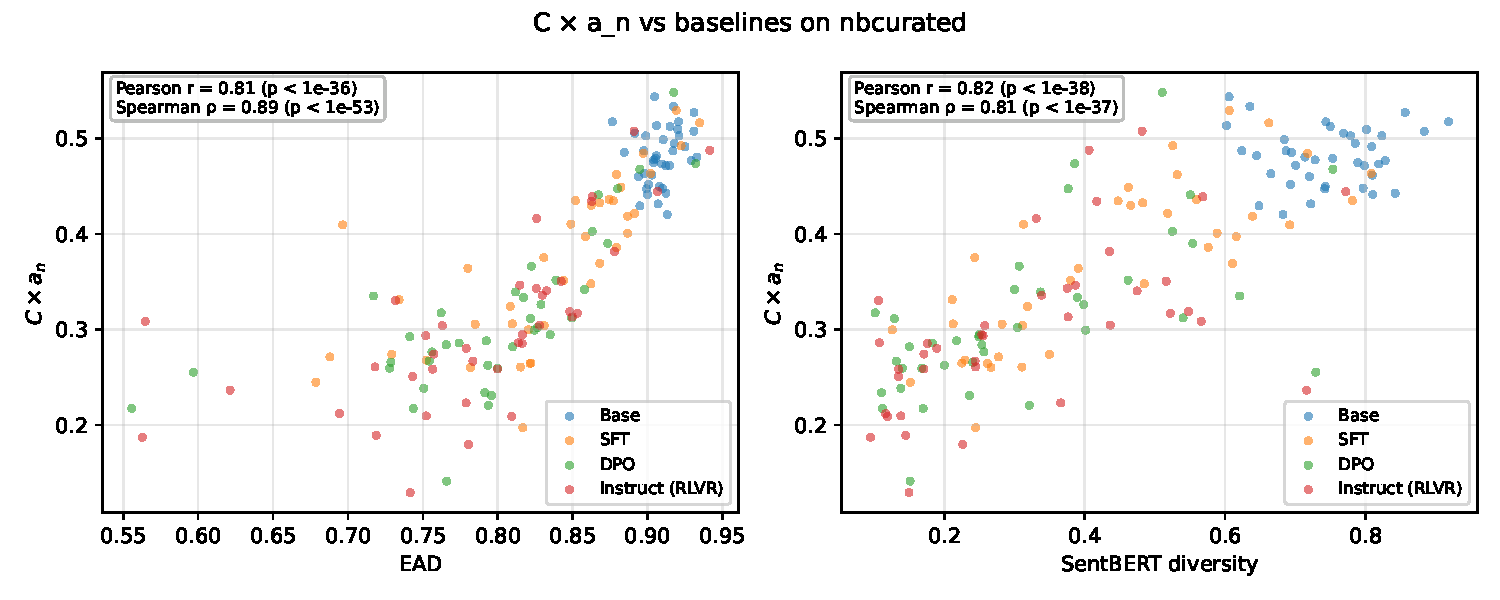
\includegraphics[width=0.85\textwidth]{../figures/rlhf_experiment/metric_correlation_scatter_nbcurated_lm.pdf}
    \caption{NoveltyBench curated (length-matched, $n=\olmoLmNbCuratedN$ prompts).}
\end{subfigure}
\caption{Per-prompt $D_{Ca_n}$ versus EAD (left subpanel) and SentBERT-similarity diversity (right subpanel), coloured by stage, on the length-matched subset of prompts. Length-matching truncates each (stage, prompt) tuple's responses to a common per-prompt byte budget so the per-byte conditional surprise that defines $a_n$ is not depressed by response length. Pearson $r$ and Spearman $\rho$ (two-sided $p$) are reported in each panel. The rank correlations are positive across both prompt sets and both baselines: $D_{Ca_n}$ tracks the same diversity-loss signal EAD and SentBERT detect, and the agreement is not an artefact of response length.}
\label{fig:rlhf-metric-scatter}
\end{figure*}
}{}


\end{document}
